\documentclass[11pt]{article}



\usepackage{deauthor}
\usepackage{enumitem}
\usepackage{algorithmic}
\usepackage{algorithm}
\usepackage{xcolor}
\usepackage{xspace}
\usepackage{graphicx}
%\usepackage[caption=false]{subfig}
\usepackage{footnote}
\usepackage{hyperref}
\usepackage{multirow}
\usepackage{subfig}
\usepackage{enumitem}
\usepackage{comment}


% Additional Package
\usepackage{times}
\usepackage{wrapfig}
\usepackage{subfig}
\usepackage{booktabs}
\usepackage{url}
\usepackage{amssymb}





% themis red comment
\newcommand{\tp}[1]{{\color{red} {\bf ??? #1 ???}}\normalcolor}
% zeyu blue answers
\newcommand{\zy}[1]{{\color{blue} {\bf - #1 -}}\normalcolor}





% \graphicspath{{Zeyu/}}


\begin{document} 


\title{Graph- and Tree-based Indexes for High-dimensional Vector Similarity Search: Analyses, Comparisons, and Future Directions}



\author{Zeyu Wang$^{\dagger}$, Peng Wang$^{\dagger}$\thanks{Corresponding author},  Themis Palpanas$^{\ddagger}$, Wei Wang$^{\dagger}$\\
$^{\dagger}$Shanghai Key Laboratory of Data Science, School of Computer Science, Fudan University\\
  \{wangzeyu17, pengwang5, weiwang1\}@fudan.edu.cn\\
  $^{\ddagger}$LIPADE, Universit{\'e} Paris Cit{\'e} \& IUF, themis@mi.parisdescartes.fr}

\setcounter{section}{0}
\setcounter{figure}{0}
\setcounter{table}{0}




\maketitle

\renewcommand\thesection{\arabic{section}}
\setcounter{section}{0}
\setcounter{figure}{0}
\setcounter{table}{0}

\begin{abstract}
Approximate nearest neighbor search on high-dimensional vectors is a crucial component for numerous applications in various fields.
To solve this problem efficiently, dozens of indexes have been proposed in the past decades.
Among them, graph-based indexes show superior query performance in memory while tree-based indexes achieve the best scalability and building efficiency.
In this paper, we systematically study the evolution of these two kinds of indexes and the recent progress with ablation studies and analyses, which help understand where the performance improvement comes from and the difference between different index families.
Moreover, we conduct a comparative study over these two index families and discuss the existing and potential combinations of them.
We believe this study can serve as a guide to the most promising directions for addressing the open problems in this area.
\end{abstract}

\section{Introduction}
% ANN, challenge, exact, approximate
% definition of the problem, metrics
% \paragraph{Background and Problem Definitions}
Approximate nearest neighbor search (ANNS) on high-dimensional vectors is a crucial component for numerous applications in various fields, such as web search engines~\cite{spann}, image retrieval~\cite{adbv}, recommendation systems~\cite{10.1145/1242572.1242610}, and large language models~\cite{openai}. 
Recent studies have further shown that deep neural networks can be augmented by retrieval to enhance accuracy on the classical problems~\cite{li2022survey} (e.g., open-domain query-answering problem~\cite{openqa}) and decrease the magnitude of parameters~\cite{pmlr-v119-guu20a}, further emphasizing the significance of ANNS in modern AI applications. Objects, such as images, documents, and videos, can be transformed into dense vectors in the embedding space. 
Given a query vector $q\in \mathbb{R}^D$ and a distance measure $dist(\cdot, \cdot)$, ANNS aims to find top-$k$ most similar objects (i.e., $kNN(q)$) in the embedding space $\mathbb{R}^D$ of the dataset.
Since the cost to find the exact $kNN(q)$ is prohibitively high, ANNS finds the approximate nearest neighbors $A(q)$ instead.
The search accuracy is measured by recall, defined as $Recall@k=\frac{1}{|Q|}\sum_{q\in Q}\frac{|A(q)\cap kNN(q)|}{k}$.
For many advanced ANNS algorithms, the recall can reach over 99\% with hundreds to thousands of times of speedup over the linear scan.
Therefore, they quickly become practical and well-recognized solutions for the applications mentioned above.

A common way of ANNS algorithms is to first build an index for the dataset and probe the index when processing queries.
In the past decades, researchers have designed dozens of index structures  to solve ANNS problems.
They can be roughly categorized into four index families: graph-based~\cite{wang-survey}, tree-based~\cite{hydra2,evolution}, quantization-based~\cite{pq} and Locality Sensitive Hashing (LSH)-based~\cite{focslsh,lsh} index family (other promising variations of these ideas have also been proposed~\cite{pdci,learnedanns}).
Although all these indexes have their specialties and advantages in certain scenarios, we focus on graph-based and tree-based indexes in this paper, because of their wide use on production systems~\cite{milvus,postgres,adbv}, and the promising future of the combination of these two techniques.

% \paragraph{Graph-based indexes.}
Graph-based indexes represent the dataset with a graph where each point is one vector.
The query processing algorithm starts from some entry point(s) and finds the approximate nearest neighbors by stepping towards the query along the edges of the graph.
With an appropriate graph structure, the search route can converge to the neighbors of the query in only a few steps, which is called the \emph{navigability} of graph-based indexes.
As extensively evaluated, graph-based indexes are the most efficient and accurate in-memory ANNS index when querying~\cite{wang-survey}.

% \paragraph{Tree-based indexes.}
Tree-based indexes on high-dimensional data are widely adopted by the industry (e.g., Postgres~\cite{postgres}, SPTAG~\cite{sptag}, ADB-V~\cite{adbv}) and famous open-source libraries (e.g., FAISS~\cite{faiss}, Scikit-learn~\cite{scikit-leran}), because of its outstanding scalability, robust performance, index-building efficiency, and high interpretability.
Classical tree-based indexes like kd-tree~\cite{kd-tree}, and ball-tree~\cite{ball-tree} suffer from the curse of dimensionality.
In high-dimensional space, simple partitioning cannot effectively cluster similar vectors.
In recent years, many classical tree indexes have been re-designed to adapt to high-dimensional space.
These indexes show the advantage on large-scale datasets for in-memory and disk indexes, stand-alone and distributed environments, as well as accuracy-guaranteed and exact $k$NN search~\cite{hydra2,elpis,spann}.
% Moreover, the strong scalability of tree-based indexes make it possible to be adapted in distributed clusters.

% \paragraph{Comparison of Graph- and Tree-based indexes.}
Although the design rationales of graph- and tree-based indexes are vastly different, we observe that there are some common design philosophies, as well as some techniques that could be complementary to each other.
As verified by results of recent studies, solving the scalability problem of graph-based index turns tractable by combining the strengths of these two kinds of indexes.
Moreover, we further propose four important open problems and directions that could be solved by this combination.

% \paragraph{Why do we compare them and make them together?}
% Open directions.

% \paragraph{Structure of this paper.}
Our paper is organized as follows.
In Section~\ref{zeyu_sec:graph}, we review the structure evolution of the graph-based index and analyzes its performance by ablation studies.
In Section~\ref{zeyu_sec:tree}, we summarize the recent progress of tree-based indexes and discuss their relationships.
In Section~\ref{zeyu_sec:compare}, we conduct a comparative study of the two kinds of indexes, %and survey the existing combination.
%After proposing four open problems, 
and discuss open research problems.
We conclude this paper in Section~\ref{zeyu_sec:conclude}.

% \section{Related Work}
% Do we need a section called "Related Work"?

% \paragraph{Other surveys and benchmarks.}

% \paragraph{Other index families}

% \emph{Quantization}

% \emph{LSH}

% \emph{Metric Index}


\section{Graph-based Index Family}
\label{zeyu_sec:graph}
% basic structure (definition), query algorithms, 
% In this section, we study the evolution of proximity graph-based high-dimensional vector index.
Graph-based index builds a directed, unweighted graph $G=(V,E)$ as the index where each vertex~\footnote{In this paper, we use vertex, node, point, and vector for graph-based indexes interchangeably.} $v\in V$ represents a vector in the dataset and the directed edge in $E$ represents some kind of proximity between two vectors.
% The query algorithm of the graph-based index follows basically the same greedy search scheme.
The widely-used greedy search algorithm starts from one or a group of entry points and approaches the query step by step. 
Two priority queues $C$ and $Res$ are maintained in this process, ordered by the distance to the query.
$C$ (with unlimited size) stores the points to be visited, while $Res$ stores only the \emph{ef} nearest points that have been checked before. 
In each step, the first point from $C$ is popped and all its out-neighbors will be checked. 
If some neighbor point's distance to the query is smaller than the furthest point in $Res$, it will be pushed into $C$ and $Res$.
The algorithm terminates when the distance of the first point in $C$ is larger than all the ones in $Res$.
Finally, the closest $k$ elements in $Res$ will be returned.
Apparently, \emph{ef} is an important parameter which controls the accuracy-efficiency trade-off.
The query processing algorithm consists of two stages~\cite{note,kbs}, a fast navigating stage leading the search route from the entry point(s) to the query's neighbors, and a recall stage that traverses the neighbors of the query to obtain the final $k$NN results.
Several extensions and improvements of this search algorithm have recently been proposed, employing query parallelization~\cite{iqan}, GPUs~\cite{song,ganns}, learned early termination~\cite{early-termination}, and guided search~\cite{kbs}.
In this section, we study the basic, common search algorithm, and focus on the structure of the graph index.





% outstanding performance
% For the first stage, the graph-based index has shown nice navigability in the literature that approaches the 1NN with logarithmic steps w.r.t. the dataset size.
% For the recall stage, since the nearest neighbors of a database point are usually linked to this point in the graph, the neighbors of the query can be obtained efficiently by traversing the neighborhood.
% As a result, the graph-based index is usually easy to achieve a high recall with only tens of search steps.
\subsection{Overview}
In this subsection, we briefly review the building process of graph-based indexes, as well as the structures they employ.
The design inheritance is shown in Figure~\ref{zeyu_fig:evo-graph}.

\paragraph{$K$-Graph~\cite{nn-descent}}
Each node in $K$-Graph out-links its $K$ nearest neighbors in the graph.
To reduce the linear complexity of index building, a dozen of accelerating techniques are proposed~\cite{nn-descent,efanna}.

\paragraph{Navigable Small World Graph (NSW)~\cite{nsw}}
NSW is built by sequential insertions of points of the dataset.
When inserting a point $v$, we find $M$ nearest neighbors on the previously-inserted sub-dataset by the greedy search algorithm.
Then NSW adds bi-directional links between $v$ and the $M$ nearest neighbors.
Note that NSW does not have a maximal out-degree limit, and the NSW index built with parameter $M$ has nearly the same number of edges as the $K$-Graph where $K=2M$.



\begin{figure}[t]
\centering
    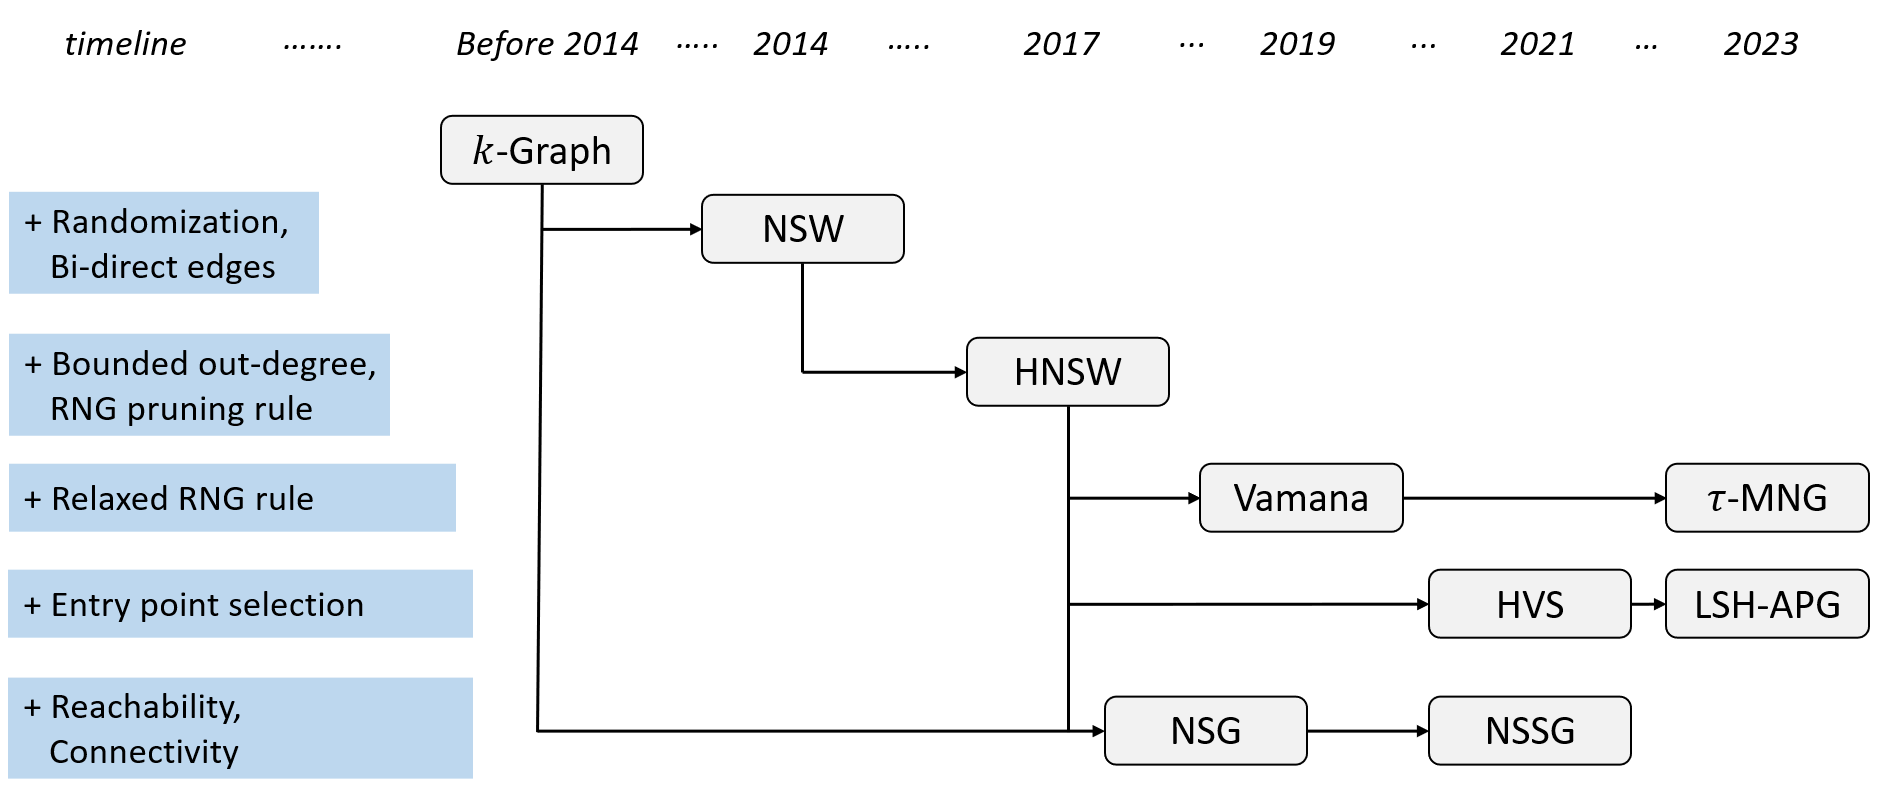
\includegraphics[width=0.8\textwidth]{submissions/Zeyu2023/figs/evo-graph.png}
    \caption{The evolution of the structures of in-memory graph-based indexes. The solid arrows denote the inheritance of designs. }
    \label{zeyu_fig:evo-graph}
\end{figure}

\paragraph{Hierarchical Navigable Small World Graph (HNSW)~\cite{hnsw}}
HNSW has a hierarchical structure where the graph in the lower layer contains all the points in the upper layers and the bottom layer HNSW$_0$ contains all points in the dataset.
The number of points is reduced exponentially bottom-up, and the level of a point is decided randomly.
The query starts from the top layer to find NNs as the entry points of the next layer until reaching the bottom layer.
Like NSW, HNSW is also built by sequential insertion and greedy search, but with a limited out-degree $2M$.
Once a point's out-degree exceeds $2M$, HNSW prunes neighbors using the RNG rule: this is derived from the Relative Neighborhood Graph~\cite{rng}.
Simply speaking, the RNG rule removes the longest edge in the triangles existing in the graph.
In this way, HNSW tries to preserve the reachability of the graph index while limiting the out-degree, by removing the ``redundant'' edges, at the expense of a few more hops when querying.

\paragraph{Relaxed pruning rule: Vamana~\cite{diskann} and $\tau$-MNG~\cite{tau}}
Since the heuristic RNG pruning rule tends to be ``strict'', recent studies have verified that some useful edges are also pruned, which leads to a sub-optimal graph structure.
Vamana relaxes the RNG rule by allowing the inclusion of the longest edge in a triangle, if it is not $1+\alpha$ times longer than the second longest edge, where $\alpha$ is a user-defined relaxing parameter.
In this way, Vamana shortens the search path when querying, which helps reduce random I/Os when the index is on disk.
A recent study~\cite{tau} points out that RNG rule is ineffective when the query does not belong to the dataset, and mitigates this problem by relaxing the RNG pruning rule with a parameter $\tau$.
We omit the details for lack of space.
The resulting approach, $\tau$-MNG, is expected to have a lower search time complexity than other graph-based indexes when the distance between the query and its nearest neighbor is smaller than $\tau$. 
% relaxes the RNG rule by a parameter $\tau$, where if the distance between two points is smaller than $3\tau$, they must connect to each other and for farther points the occlusion area is also narrowed.
% $\tau$-MNG is expected to have better navigability where each step in the search route is closer to the query by $\tau$ under some circumstances.

\paragraph{Better entry points: HVS~\cite{hvs} and LSH-APG~\cite{lsh-apg}}
HVS and LSH-APG use auxiliary data structures to obtain better entry points for the graph-based indexes.
HVS leverages an adaptive hierarchical tree index with quantization techniques, while LSH-APG builds multiple LSB-trees for coarse-grained indexing.
The graph-based index is HNSW$_0$~\cite{hvs}, or even a simpler variant~\cite{lsh-apg}.

\paragraph{Better reachability: NSG~\cite{nsg} and NSSG~\cite{nssg}}
Although HNSW achieves prominent \emph{average} query performance, it cannot guarantee the reachability to any point in the graph index.
Since accomplishing the reachability starting from any point in the graph is intractable, recent graph-based indexes opt to fix the entry point(s) and guarantee the reachability from these entry points.
NSG uses the medoid point of the dataset as the entry point, and refines $K$-Graph to ensure reachability.
Specifically, for a specific point $v$, NSG regards $v$ as a query and performs approximate greedy search in the graph index.
The visited points during the search (along with the neighbors of $v$ in $K$-Graph) become the candidate neighbors of $v$, and are then pruned by RNG rule to limit the out-degree.
After iterating all the points, NSG tests the reachability with a Deep-First-Search Tree rooted at the entry point.
The isolated points will be linked by the nearest point in the tree.
In contrast to NSG, NSSG randomly selects a group of points as entry points, and only uses two-hop neighbors of a point in $K$-Graph as the candidates of neighbors for pruning.
Besides the reachability to the point in the dataset, NSSG also considers the points that do not belong to the dataset, by studying the trade-off between the navigability and the sparsity of the graph index under the RNG rule.
% NSG extends the candidate neighbors by searching $k$NN on existing graphs and uses the RNG rule to prune neighbors like HNSW.
% Furthermore, to ensure connectivity, NSG performs a DFS from the entry point as the root node and adds a link for the point that cannot be reached from the nearest neighbors of the point in the DFS-Tree.~\footnote{todo: decompose}
% In contrast to NSG, NSSG takes two-hop neighbors in $K$-Graph as candidates and tries to add reversed edges for more long-range connections.

\subsection{Understanding the Evolution with Ablation Studies}
Although the heuristics of advanced graph-based indexes have been stated in the papers, it is yet not clear why the proposed techniques work well.
In this subsection, we describe the evolutionary process from $K$-Graph to NSW, HNSW and more optimizations on HNSW by abundant ablation studies.
We aim to help readers understand which techniques actually enhance the performance and the reasons behind their effectiveness from a novel perspective, which can inspire the future designs of ANNS algorithms.

\subsubsection{The problem of $K$-Graph}
\label{zeyu_sec:k-graph}
\begin{wraptable}{r}{0.36\textwidth}
        \centering
        \footnotesize
    \caption{Skewness of in-degree distribution of graph-based indexes}
    \label{zeyu_tab:skewness}
    \begin{tabular}{ccc}\\
    \toprule
              & Deep1M & SIFT1M \\ \midrule
    $K$-Graph & 2.436  & 1.875  \\ \midrule
    NSW       & 4.642  & 4.107  \\ \midrule
    pNSW      & 4.025  & 3.457  \\ \midrule
    HNSW$_0$   & 1.209  & 1.395  \\ \bottomrule
    \end{tabular}
\end{wraptable}
We start by examining the $K$-Graph approach, because not only $K$-Graph is a graph-based index, but it also exhibits some inherent properties (detailed below) of high-dimensional vectors in the context of ANNS problem. 
In this paper, we use \emph{exact} $K$-Graphs instead of approximate ones to avoid the effect of approximation errors.
A common argument in the literature for the unsatisfactory query performance of $K$-Graph is the loss of navigability~\cite{hnsw,wang-survey}, which is verified on real datasets in ~\cite{k-regular}.
However, it is not yet clear the root cause of the loss of navigability.
According to previous studies, the distribution of in-degree of points is very skewed~\cite{hub}.
That is, a small portion of points occupy most of the $k$NN lists for all the points while most of the other points are rarely linked by others.
This is also verified by our experiments on real datasets as shown in Table~\ref{zeyu_tab:skewness} with skewness (standardized third moment).
For simplicity, we denote the in-degree of a point in $K$-Graph by $k$-occurrence~\cite{hub}.
Note that $k$-occurrence is a property of a point in a dataset, independent of the type of index built on the dataset.

Furthermore, we observe that in $K$-Graph the points with high in-degree (i.e., hubs) always interconnect with each other.
To describe this phenomenon, we define the out-link density of a group of points $X\subset V$ as $\rho_{out-link}(X) = \frac{|\{(x,y)|x, y\in X \wedge (x,y)\in E\}|}{|\{(x,y)|x \in X \wedge y \in V \wedge (x,y)\in E\}|}$.The out-link density describes how much a group of points is interconnected.
A high out-link density means these points tend to connect to themselves rather than other points in the graph.
In Figure~\ref{zeyu_fig:outlink-density}, we select different number of hubs and compute the average out-link density of these hubs.
The baseline is a random graph, where each point has $K$ out-neighbors selected uniformly at random. 
As we can see, the out-link density of the hubs in $K$-Graph is much higher than the random graph and NSW.
Over half of the out-links of the 5\% hubs connect to themselves instead of other points.
\begin{wrapfigure}{r}{0.64\textwidth}
    \centering
    \subfloat[Deep1M]{
    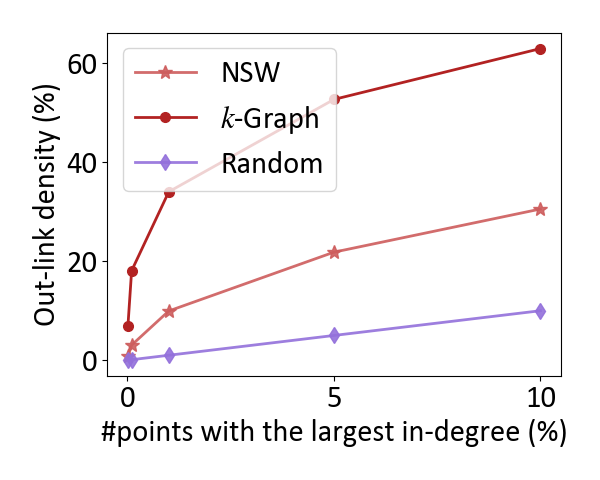
\includegraphics[width=0.32\textwidth]{submissions/Zeyu2023/figs/deep-outlink-density.png}
    \label{zeyu_fig:outlink-density-deep}
    }
    \subfloat[Sift1M]{
    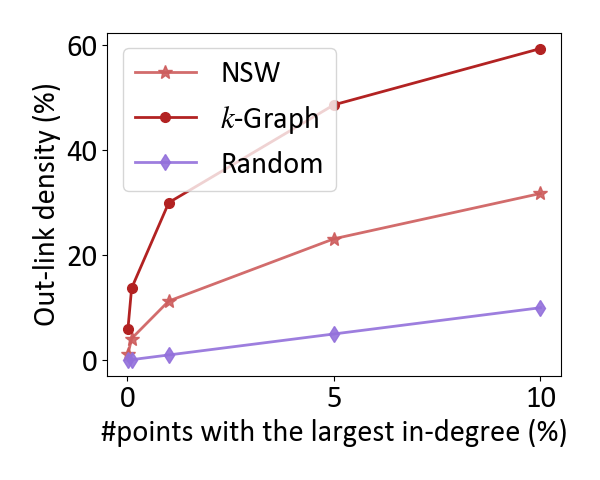
\includegraphics[width=0.32\textwidth]{submissions/Zeyu2023/figs/sift-outlink-density.png}
    \label{zeyu_fig:outlink-density-sift}
    }
    \caption{Out-link density of the group of points with the largest in-degree.}
    \label{zeyu_fig:outlink-density}
\end{wrapfigure}

This phenomenon leads to local optima in $K$-Graph, which is a classical problem of the greedy search algorithm.
Consider an extreme case where $ef=1$ for querying, i.e., $Res$ only contains the nearest checked point to the query, which means that the points further than the current visited point will never be visited.
In other words, no backtracking exists in the search route.
In this case, if the search route steps into a point which is closer to the query than all its neighbors, the search algorithm terminates directly, as shown in Figure~\ref{zeyu_fig:local-optimum}, and the actual nearest neighbors (that could be reached by detouring) are missed.
The termination point is a local optimum, in contrast to the global optimum (i.e., real $k$NN).
\begin{wrapfigure}{r}{0.36\textwidth}
    \centering
    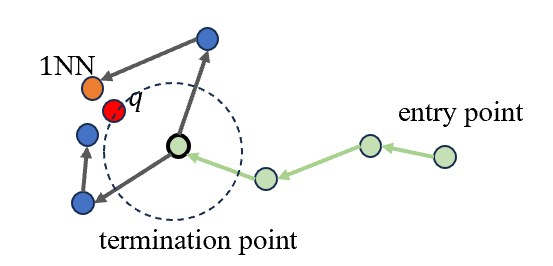
\includegraphics[width=0.36\textwidth]{submissions/Zeyu2023/figs/local-optimum.png}
    \caption{An example of local optimum in the greedy search algorithm.}
    \label{zeyu_fig:local-optimum}
\end{wrapfigure}
Since in $K$-Graph, most of the out-neighbors of a hub are also hubs, once the search route steps into one hub, it is hard to escape from the local optimum to other regions, which may actually contain the true nearest neighbors.
Worse still, the hubs are frequently visited when querying since the points with high in-degree have a higher probability to be visited when starting from a random point.
As a result, $K$-Graph shows weak navigability to acquire real $k$NN even with a large $ef$.

We further verify this impact by analyzing the returned results of the greedy search algorithms.
Formally, given a query $q$, we collect the true positive set $S_{TP} = A(q) \cap kNN(q)$, the false positive set $S_{FP} = A(q) - kNN(q)$ and the false negative set $S_{FN} = kNN(q) - A(q)$, and compute the average $k$-occurrence of these point sets, denoted by $k^{occur}_{S_{TP}}$, $k^{occur}_{S_{FP}}$ and $k^{occur}_{S_{FN}}$, respectively.
% Recall that the properties on $K$-Graph, as we mentioned at the beginning, are at the same time the properties of the distribution of the data.
In the experiments, we use the same query algorithm and the same sparsity of the graphs with $K$=32 for $K$-Graph and $M$=16 for the other three.
As shown in Table~\ref{zeyu_tab:query-analyses}, for $K$-Graph, the difference between $k^{occur}_{S_{TP}}$ and $k^{occur}_{S_{FN}}$ is the largest, indicating that the points with higher in-degree are easier to be recalled whereas the missing points are markedly less connected.
Moreover, the average $k$-occurrence of points in $S_{FP}$ is also higher than $S_{FN}$ for $K$-Graph, and to achieve a higher recall (95\%), $K$-Graph needs the most number of steps compared with other indexes.
These results verify the above inference that the search route in $K$-Graph is prone to get stuck in the local optimum formed by the hubs and thus needs to pay more effort to escape from this trap.

\begin{table}[t]
\centering
\footnotesize
\caption{Average $k$-occurrence of different sets returned by the greedy search algorithm on different graph-based indexes. \#hops are the average number of points visited in the search route. NDC stands for the average Number of Distance Calculations during search, which represents the time cost.}
\label{zeyu_tab:query-analyses}
\begin{tabular}{ccccccccc}\\
\toprule
Dataset              & Accuracy & Index    & $k^{occur}_{S_{TP}}$    & $k^{occur}_{S_{FP}}$    & $k^{occur}_{S_{FN}}$    & $k^{occur}_{S_{TP}} - k^{occur}_{S_{FN}}$ & \#hops & NDC  \\ \midrule
\multicolumn{1}{c}{\multirow{8}{*}[-6.5mm]{Deep1M}} & \multirow{4}{*}[-3mm]{recall@50=0.90} & $K$-Graph & 61.08 & 41.86 & 14.44 & 46.64 & 116 & 1716 \\ \cmidrule{3-9}
\multicolumn{1}{c}{} &          & NSW      & 61.06 & 40.72 & 32.99 & 28.07   & \textbf{57}     & 1709 \\\cmidrule{3-9}
\multicolumn{1}{c}{} &          & pNSW     & 62.15 & 46.36 & 24.66 & 37.49   & 90     & 1379 \\\cmidrule{3-9}
\multicolumn{1}{c}{} &          & HNSW$_0$ & 61.00 & 45.46 & 37.05 & \textbf{23.95}   & 79     & \textbf{1287} \\\cmidrule{2-9}
\multicolumn{1}{c}{}                        & \multirow{4}{*}[-3mm]{recall@50=0.95} & $K$-Graph & 60.38 & 27.30 & 7.62  & 52.76 & 176 & 2319 \\\cmidrule{3-9}
\multicolumn{1}{c}{} &          & NSW      & 60.17 & 28.28 & 19.55 & 40.62   & \textbf{108}    & 2734 \\\cmidrule{3-9}
\multicolumn{1}{c}{} &          & pNSW     & 61.22 & 31.96 & 15.37 & 45.85  & 162    & 2170 \\\cmidrule{3-9}
\multicolumn{1}{c}{} &          & HNSW$_0$ & 60.72 & 32.57 & 24.39 & \textbf{36.33}   & \textbf{108}    & \textbf{1781} \\\cmidrule{1-9} \cmidrule{1-9}
\multirow{8}{*}[-6.5mm]{SIFT1M}                     & \multirow{4}{*}[-3mm]{recall@50=0.90} & $K$-Graph & 53.81 & 28.90 & 11.72 & 42.09 & 386 & 4927 \\\cmidrule{3-9}
                     &          & NSW      & 54.07 & 41.78 & 37.86 & 16.21   & \textbf{70}     & 2015 \\\cmidrule{3-9}
                     &          & pNSW     & 54.98 & 45.44 & 31.84 & 23.14   & 106    & 1690 \\\cmidrule{3-9}
                     &          & HNSW$_0$ & 54.18 & 44.40 & 40.10 & \textbf{14.08}   & 71     & \textbf{1336} \\\cmidrule{2-9}
                                            & \multirow{4}{*}[-3mm]{recall@50=0.95} & $K$-Graph & 52.86 & 37.27 & 17.17 & 35.69 & 423 & 5336 \\\cmidrule{3-9}
                     &          & NSW      & 54.03 & 32.77 & 27.71 & 26.32   & 112    & 2881 \\\cmidrule{3-9}
                     &          & pNSW     & 54.55 & 35.59 & 23.01 & 31.54   & 169    & 2464 \\\cmidrule{3-9}
                     &          & HNSW$_0$ & 54.03 & 34.04 & 29.70 & \textbf{24.33}   & \textbf{108}    & \textbf{1890}\\\bottomrule
\end{tabular}
\end{table}


Recall that the problems of $K$-Graph is an intrinsic problem for all graph-based indexes on high-dimensional data.
% The dilemma is between local proximity and global navigability.
On the one hand, the local proximity of $K$-Graph is crucial in the recall stage during the search process~\cite{note}.
On the other, over-rich local connections in the graph lead to more local optimum which hinders the search accuracy.
% The global navigability can be achieved by diversified edges in different lengths and directions, which however, turn to be burdens on the recall stage.
% In the following, we will show how the following works face this dilemma and improve the overall performance of the index. 
\begin{table}[tb]
\begin{minipage}{.4\linewidth}
    % \centering
    \footnotesize
        \caption{Pearson correlation coefficients between in-degree and insertion-order/$k$-occurrence of points on different indexes.}
    \begin{tabular}{ccccc}\\
\toprule
& \multicolumn{2}{c}{Deep1M} & \multicolumn{2}{c}{Sift1M} \\\midrule
& Ins. ord.     & $k$-occur.    & Ins. ord.     & $k$-occur.    \\\midrule
$K$-Graph & 0.00  & 1.00 & 0.00 & 1.00  \\ \midrule
NSW       & -0.53  & 0.56 & -0.53 & 0.56  \\ \midrule
pNSW      & -0.44  & 0.68 & -0.43 & 0.67 \\ \midrule
HNSW$_0$   & -0.63  & 0.22 & -0.52 & 0.26  \\ \bottomrule \\
\end{tabular}
    \label{zeyu_tab:corr}
\end{minipage}%
\hspace{6mm}
\begin{minipage}{.31\linewidth}
    \centering
    \footnotesize
    % \scriptsize
     \caption{Query analyses under recall@1=99\%, on different graph-based indexes.}
\begin{tabular}{cccc}\\
\toprule
 \multicolumn{2}{c}{Deep1M} & \multicolumn{2}{c}{Sift1M} \\\midrule
 \#hops     & NDC    & \#hops     & NDC  \\\midrule
  5001  & 29315 & 2047 & 17698  \\ \midrule
        137  & 3244 & 150 & 3644  \\ \midrule
      156  & 3074 & 663 & 7246 \\ \midrule
    156  & 2422 & 111 & 1943  \\ \bottomrule \\
\end{tabular}   
    \label{zeyu_tab:high-recall}
\end{minipage}%
\hspace{2mm}
\begin{minipage}{.22\linewidth}
    \centering
    \footnotesize
    % \scriptsize
\caption{Graph quality of different indexes, where $K$=32 and $M$=16}
\begin{tabular}{cc}\\
\toprule
          Deep1M & Sift1M \\ \midrule
          GQ & GQ \\\midrule
 100\%  & 100\%  \\ \midrule
 51.84\%  & 53.76\%  \\ \midrule
51.82\%  & 52.71\%  \\ \midrule
30.80\%  & 32.17\%  \\ \bottomrule \\
\end{tabular}
    \label{zeyu_tab:graph-quality}
\end{minipage}%
\end{table}

\subsubsection{The Benefit of Long-range Connections}

%Traditional view is small-world graph
% But now we explain it from the hubness
% more tractbale, more comprehensive
% provide a novel view to understand it
% overcome hubness is not easy: recall stage and trap
% conclusion: randomize incur long edges
To mitigate the problem of $K$-Graph, NSW introduces long-range connections to break the traps formed by hubs, and enhance global navigability.
The long-range connections can be defined as the edges that do not exist in the $K$-Graph (whose graph sparsity is similar to NSW).
NSW introduces these connections by randomization.
Recall that when inserting a point, NSW finds its nearest neighbors by greedy search on the \emph{existing} graph, and then builds bi-directional links with these neighbors.
In this way, the degree~\footnote{Note that in NSW, the \emph{in-degree} of a point is equal to its \emph{out-degree} since all edges are bi-directional. Thus, we simply use the term \emph{degree}.} of points in NSW is significantly influenced by the insertion order: the points inserted earlier have a higher possibility to be linked by other points than the later ones.
This is demonstrated in Table~\ref{zeyu_tab:corr}, where the NSW (second line) Pearson correlation coefficients for $k$-occurrence and insertion order are (almost) the same.  
Given that the insertion order is usually random, the lengths of the new links introduced in NSW also tend to be random.
Thus, long-range connections are introduced.

We quantify the size of long-range connections by graph quality~\cite{k-regular,wang-survey}, which is defined as the overlapping ratio of edges with $K$-Graph under similar sparsity.
As shown in Table~\ref{zeyu_tab:graph-quality}, NSW preserves nearly half of the short edges belonging to $K$-Graph, while introducing long-range connections for the other half.
Although affected by the random selection of the previously inserted points, these connections can substantially improve the navigability of graph indexes, as we explain below.
We note that the hubs do not necessarily have high $k$-occurrence, but are also determined by the insertion order.
In other words, the distribution of hubs is ``disrupted'' by randomization.
As a result, the hubs in NSW are not interconnected, and the out-link density of hubs significantly drops compared to $K$-Graph (see Figure~\ref{zeyu_fig:outlink-density}).
It means that although the hubs are still visited frequently, the cases of local optimum are reduced and thus the navigability on NSW is enhanced.
% In contrast to $K$-Graph where the in-degree only relates to $k$-occurrence as defined, in NSW, the insertion order has nearly the same influence as $k$-occurrence on the in-degree of nodes, as shown in Table~\ref{zeyu_tab:corr}.
% Since the insertion order is random in NSW, it can be viewed that the influence of hubness is ``disrupted'' by randomization.
% As a result, the new hubs in NSW are not necessarily close to a large number of points.
% Also, in Figure~\ref{zeyu_fig:outlink-density}, we can see a significant drop from $K$-Graph to NSW w.r.t. out-link density, which means the interconnection of the hubs is weakened.
% In this way, NSW breaks the local optimum formed by the hubs and enhances the navigability.

% In addition, NSW also preserves the local proximity by adding the reversed edges.
% It can be proved that the bi-directional $k$NN of a point $v$, defined as $\{x|x\in kNN(v) \wedge v\in kNN(x)\}$, will be $v$'s neighbors in NSW, {\color{red}under the assumption that the greedy search during constructing NSW is accurate}.

% {\footnote{todo: what does this paragraph mean? it's not clear}}
% Table~\ref{zeyu_tab:graph-quality} shows that the graph quality~\cite{wang-survey,k-regular}~\footnote{todo:add definition of graph quality} of NSW is over 50\%, indicating that over half of the edges in $K$-Graph are preserved in NSW.
Table~\ref{zeyu_tab:query-analyses} shows that in order to achieve the same recall, NSW needs on average only \textbf{32}\% of the $K$-Graph steps.
The difference between $k^{occur}_{S_{TP}}$ and $k^{occur}_{S_{FN}}$ is reduced by half, clearly demonstrating that the missing nearest neighbors are less susceptible to local optima, and leading to performance improvements. % beyond $K$-Graph on some settings, verifying our analyses beforehand.
In some cases though, e.g., in the Deep1M dataset, the improvement is marginal and even negative, despite the short search paths.
The reason is that the degree of NSW is not fixed.
Since the search cost of the greedy search algorithm is the product of the length of the search route and the out-degree of each point in the route, a high out-degree will linearly increase the time complexity.
Worse still, the distribution of degree of points in NSW is even more skewed than $K$-Graph (see Table~\ref{zeyu_tab:skewness}), which further degrades the worst-case time complexity.

% not necessarily with low $k$-occurrence; NSW is not trapped by interconnected hubs, despite that the search algorithm still shows bias on points with high $k$-occurrence.

% {\footnote{todo: pNSW is for the benefit of long-range connections}}
% Although NSW provides better navigability than $K$-Graph, a nice property that {\footnote{todo:rewrite}} the out-degree of each node is fixed, is violated.
% It leads to the distribution of out-degree (equally to in-degree) is severely skewed in NSW, as shown in Table~\ref{zeyu_tab:skewness}.
% Since the search cost of the greedy search algorithm is the product of the length of the search route and the out-degree of each point in the route, a high out-degree will linearly increase the time complexity.
% {\footnote{todo: why NSW is not good, table 2}}

A simple optimization is to restrict the out-degree to $2M$ by selecting the nearest $2M$ neighbors.
We call this method pruned-NSW (pNSW).
pNSW mainly removes the long-range connections, which can be verified by the fact that the graph quality is nearly the same as NSW (see Table~\ref{zeyu_tab:graph-quality}).
% The graph quality of pNSW is nearly the same as NSW (see Table~\ref{zeyu_tab:graph-quality}), verifying that the local proximity remains unchanged.
As shown in Table~\ref{zeyu_tab:query-analyses} pNSW seems have a better performance than NSW by sacrificing a little navigability and achieves a remarkable gain in overall performance.
However, as shown in Table~\ref{zeyu_tab:high-recall}, under high-recall constraint (99\% recall@1), pNSW suffers a significant degradation on Sift1M dataset, nearly two times slower than NSW.
The results of pNSW further demonstrate that the long-range connections, especially the links of the hubs, significantly influence the global navigability of the graph index.
% It results from the reduction of long-range links.
% However, the reduction of long-range links, especially the links coming from the hubs, significantly impairs global navigability.
% \begin{wrapfigure}{r}{0.38\textwidth}
%     \centering
%     \includegraphics[width=0.38\textwidth]{figs/triangle.png}
%     \caption{Tree design principles of graph-based indexes.}
%     \label{zeyu_fig:triangle}
% \end{wrapfigure}

% The results of pNSW inspire us that an efficient graph-based index 
% Therefore, the technical challenge lies in the triangle that what will be the optimal edge allocation strategy that satisfies local proximity, global navigability and low out-degree at the same time, as shown in Figure~\ref{zeyu_fig:triangle}.
% To overcome this challenge, it is intuitive to satisfy the low out-degree by a fixed parameter, and then balance the local proximity and navigability given the limited edge budget.

\subsubsection{The RNG Pruning Rule}
Up to this point, there seems to exist a tradeoff in the design of graph indexes between search efficiency and navigability.
If we limit the (out-)degree of points for efficiency, navigability will be hurt, as in $K$-Graph and pNSW.
If we break the degree limit, the search efficiency will degrade, as in NSW.
To address this situation, we observe that the distribution skewness of the points' in-degree is a key point.
A skewed distribution means the existence of hubs in the graph, and given the high visit frequency of these hubs, these hubs bear the responsibility of high navigability.
In order to provide navigability, hubs need a high degree and more long-range connections, causing the problem mentioned above.
Therefore, if we can render in-degree distribution less skewed, then hubs will no longer exist and the navigability will be provided equally by all the points in the graph.
In this case, the bounded degree and the navigability can be achieved at the same time.

HNSW is a nice example of this rationale.
Given that the skewness of the $k$-occurrence distribution is an inherent property of high-dimensional vectors, ``amortizing'' the navigability to all points is very challenging.
HNSW leverages two techniques to accomplish this target.
One is randomization, like NSW, which disrupts the distribution of hubs.
The other is RNG pruning rule, which is a key design inherited by most of the following graph-based techniques~\cite{nsg,nssg,wang-survey}.
Specifically, for a point $v$ to be inserted, HNSW first collects sufficient nearest neighbors on the existing graph as candidates by greedy search, and then prunes these candidate neighbors down to $M$, using the RNG rule.
Finally, like NSW, HNSW tries to add $M$ reversed links from the $M$ selected neighbors to $v$.
Once the reversed link exceeds the out-degree limit $2M$, the RNG rule will be used to prune these neighbors to no more than $2M$.
For clarity, we only consider HNSW$_0$ in this section to avoid the influence of the hierarchy, which will be discussed separately in the next section.

When pruning candidate neighbors, HNSW sorts them according to the distance to the inserted point $v$ and checks them in order.
The inserted neighbor $c$ should satisfy that $\forall c'\in C(v), dist(v,c)<dist(c,c')$, where $C(v)$ is the set of already selected neighbor points. 
Consider the example in Figure~\ref{zeyu_fig:rng} (left), where $C=\{c_1,c_2\}$.
The next candidate neighbor $c$ will be pruned, because $dist(v,c)>dist(c,c_2)$.
The heuristic behind the RNG rule is that for the pruned neighbors like $c$, even though $v$ does not directly link to $c$, $v$ can reach $c$ by detouring from $c_2$.
Since $c_2$ is closer to $c$, $v$ must not be the local optimum if the query is on, or near to $c$.
As a result, compared to NSW, HNSW filters out many of the $M$ nearest neighbors found during the greedy search, without losing the reachability to them~\footnote{This is not strict since there is no guarantee on the existence of edge ($c_2,c$).}.
In this way, the saved slots of out-neighbors can be used to accommodate more long-range connections. 
As shown in Table~\ref{zeyu_tab:graph-quality}, only about 30\% of the edges in $K$-Graph are preserved in HNSW. 

\begin{wrapfigure}{r}{0.36\textwidth}
    \centering
    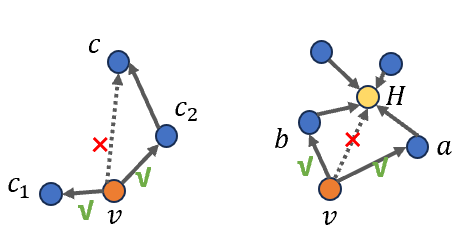
\includegraphics[width=0.36\textwidth]{submissions/Zeyu2023/figs/rng.png}
    \caption{RNG rule.}
    \label{zeyu_fig:rng}
\end{wrapfigure}


Besides pruning some ``unnecessary'' edges, the RNG rule also helps mitigate the skewness of in-degree distribution for high-dimensional vectors.
Specifically, the points with high $k$-occurrence tend to reject more in-links from other points because of the RNG rule.
Consider the example in Figure~\ref{zeyu_fig:rng} (right), where $C(v)=\{a,b\}$, and the candidate neighbor $H$ has been linked by some points because of closeness.
In this case, $H$ will be pruned since it can be reached indirectly from $a$ and $b$.
This example indicates that if a point is close to many other points (i.e., points with high $k$-occurrence like $H$), it has to ``compete'' against these close points for becoming the neighbor of an inserted point.
Naturally, the probability of building links with such points is lower than the point with low $k$-occurrence.
This is exactly the opposite to the linking strategy of the $K$-Graph index.
As shown in Table~\ref{zeyu_tab:corr}, the correlation coefficient between the in-degree and $k$-occurrence for HNSW is less than 0.3, indicating a very weak correlation.
As a result, the inherent skewness of the in-degree distribution of high-dimensional vectors is optimized by the RNG rule: the skewness value drops to nearly a half when compared to $K$-Graph, as shown in Table~\ref{zeyu_tab:skewness}. 
% In this way, the difference of visit frequency among the points in the graph is not outstanding and the navigability is achieved by all the points. 
Moreover, for every point in HNSW, there exists a sufficient number of short edges for local proximity, but also enough long-range connections for global navigability, which ensure the query efficiency in the recall and navigation stage respectively.
As shown in Tables~\ref{zeyu_tab:query-analyses} and~\ref{zeyu_tab:high-recall}, even though HNSW has a limited out-degree, it uses a similar number of steps to NSW in order to reach a low/high recall.
This demonstrates that the RNG rule successfully preserves the navigability in these datasets.
As for the overall query performance, HNSW always achieves the best results (well ahead of the second best), across all settings.  

% and the current point $x$ that regards $H$, $a$ and $b$ as candidates of neighbors.
% When selecting neighbors, the nearest $a$ is first selected and then $b$ is also selected since $b$ is closer to $x$ than to $a$.
% The third candidate is $H$, which will be rejected since $x$ can already access $H$ by $a$ or $b$.
% In addition, RNG rule also effectively mitigates the skewness of the in-degree distribution, a significant drop as shown in Table~\ref{zeyu_tab:skewness}.
% Specifically, the points with high $k$-occurrence tend to reject more in-links from other points due to RNG rule.
% As we have described in Section~\ref{zeyu_sec:k-graph}, the hubs are usually close to many other points.
% Consider the point $H$ in Figure~\ref{zeyu_fig:rng} that has been linked by some points, and the current point $x$ that regards $H$, $a$ and $b$ as candidates of neighbors.
% When selecting neighbors, the nearest $a$ is first selected and then $b$ is also selected since $b$ is closer to $x$ than to $a$.
% The third candidate is $H$, which will be rejected since $x$ can already access $H$ by $a$ or $b$.
% Therefore, more old hubs from $K$-Graph are removed, and the points far from the center, in a relative sense, obtain more opportunities to absorb links from other points.
% This result is consistent with our inference above that achieving low out-degree and navigability requires less skewed distribution and fewer hubs.
% As a result, HNSW allows more effective long-range connections for navigability (see Table~\ref{zeyu_tab:high-recall}), and preserves the efficiency in the local recall stage (see Table~\ref{zeyu_tab:query-analyses}).




% An inspiration from pNSW is that once the out-degree is bounded, the navigability of any point in the graph is also bounded, including the hubs that provide the function of navigability in NSW.
% To overcome the trade-off between low out-degree and navigability, a latent requirement is that the skewness of in-degree distribution should be weakened.
% In this case, the function of navigability should be transferred equally to all the points in the space, that is, the hubs no longer exist.

% \footnote{todo: HNSW does what I say before}
% In HNSW, the RNG-based pruning rule is used to remove unnecessary edges in the graph, especially in the local neighborhood of a point, and thus leaves more space for long-range connections.
% The core technique of HNSW is the RNG-based pruning rule (RNG rule for short).
% \footnote{todo: cannot get why short edges are removed}
% Simply speaking, given the nearer neighbors are considered first, RNG rule removes the longest edge in any triangle of the graph, as shown in Figure~\ref{zeyu_fig:rng}.
% ~\footnote{rewrite the follwing sentence}
% The heuristic is that the current node, though cannot visit the removed neighbors directly, can access them by a hop of existing neighbors.
% In this way, HNSW preserves the local proximity with much fewer edges, about 30\% of slots as shown in Table.~\ref{zeyu_tab:graph-quality} at the cost of several additional hops.
% The same heuristic also holds for the pruning of long-range links, allowing longer and diversified connections to enhance navigability.



\subsubsection{Hierarchy and Selection of Entry Points}
The classical hierarchical index structure of HNSW is widely employed in both research and industrial settings~\cite{k-regular,diskann,nsg,milvus}.
Intuitively, the upper layers in HNSW form long-range connections providing navigability, while the bottom layer uses small-range links to cover ``the last mile''.
However, we claim that this strategy does not provide any significant benefits in the case of high-dimensional spaces.
As shown in Figure~\ref{zeyu_fig:ablation}, using HNSW$_0$ (the bottom layer of HNSW) alone, leads to nearly the same query performance as (the original, hierarchical) HNSW. 
This result, which is verified on a dozen of public datasets (omitted due to lack of space) as well as by other studies~\cite{promise}, casts some doubt about the usefulness of the hierarchical structure.
We make the following two observations that try to explain the above result:
% \begin{itemize}
(i) Due to the distance concentration phenomenon~\cite{dist-concentrate}, the query is not far away from a random point in the same dataset.
For example, in Sift1M and Deep1M datasets, the average distance between a random point and the query is merely \textbf{5.3}x and \textbf{3.5}x, respectively, larger than the average length of the short edges in $K$-Graph.
(ii) The bottom layer can provide the navigability necessary to quickly approach the local neighborhood.
For example, to achieve 99\% recall@1, HNSW$_0$ needs 111 hops on the Sift1M dataset, compared to 108 hops for HNSW; on Deep1M, HNSW$_0$ needs 156 hops, compared to 151 hops for HNSW.
These small differences verify the efficient navigability of HNSW$_0$.
% \end{itemize}

% \begin{wrapfigure}{r}{0.3\textwidth}
%     \centering
%     \includegraphics[width=0.3\textwidth]{figs/upper-layer.png}
%     \caption{Quality of entry points in HNSW.}
%     \label{zeyu_fig:upperlayer}
% \end{wrapfigure}
\begin{figure}[tb]
    \centering
    \subfloat[Sift1M]{
    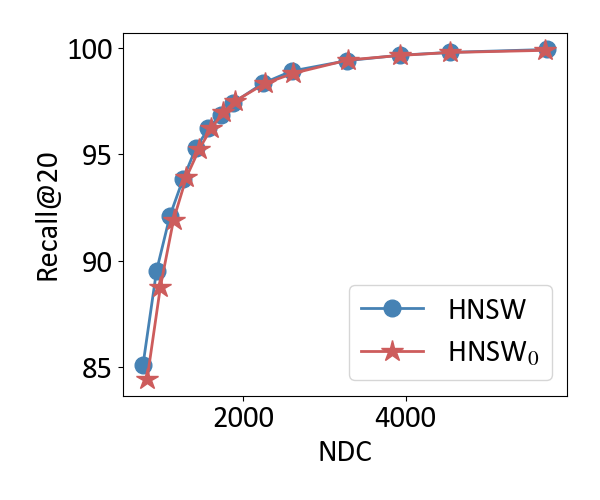
\includegraphics[width=0.33\textwidth]{submissions/Zeyu2023/figs/sift-upper-layer.png}
    }
    \subfloat[Deep1M]{
    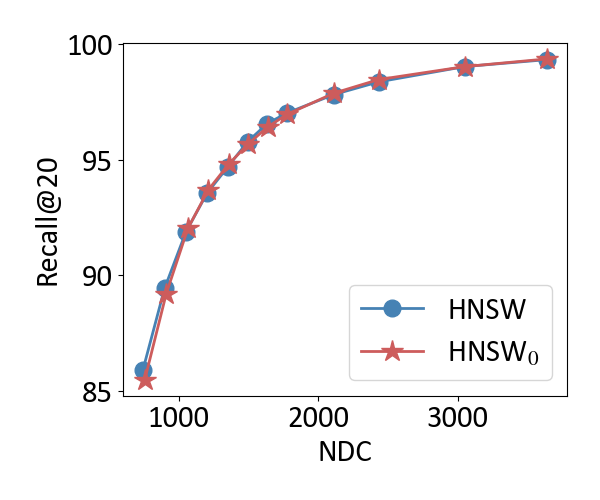
\includegraphics[width=0.33\textwidth]{submissions/Zeyu2023/figs/deep-upper-layer.png}
    \label{zeyu_fig:ndc-deep}
    }
    \subfloat[Deep10M]{
    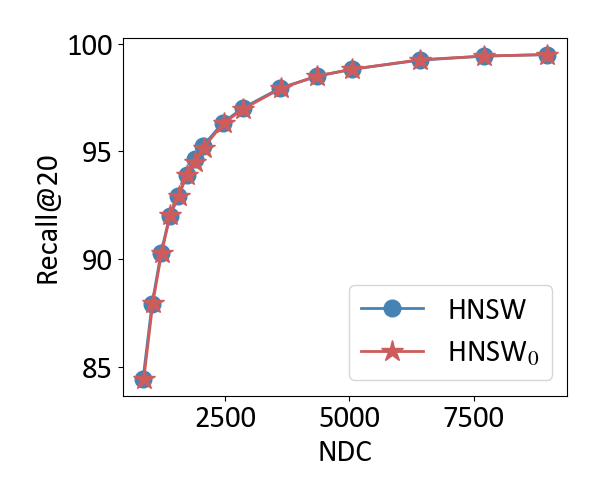
\includegraphics[width=0.33\textwidth]{submissions/Zeyu2023/figs/deep10M-upper-layer.png}
    \label{zeyu_fig:ndc-deep10M}
    }
    \caption{The query performance of HNSW and HNSW$_0$: the difference is negligible.}
    \label{zeyu_fig:ablation}
\end{figure}
In this case, the benefit of the selection of entry points for graph-based indexes relies on the accuracy of the entry points and the cost of obtaining these entry points.
Unfortunately, the upper layers of HNSW do not show an obvious benefit since they only contain a small portion of data.
According to our experiments, only less than half of the queries obtain one of the 50NN in the upper layers, which means that a significant part of the work actually takes place at the bottom layer. 
To break this limit, subsequent works, including HVS~\cite{hvs} and LSH-APG~\cite{lsh-apg} (both discussed earlier), use another index as an auxiliary structure to help obtain high-quality entry points.
% Certainly, the auxiliary index contains all the points of the dataset and is able to quickly acquire approximate $k$NN which are good enough to act as the entry points for HNSW$_0$.
The quality of entry points is largely improved, and as reported, HVS achieves over 3x faster query answering time than HNSW on hard datasets and high recall range, while LSH-APG achieves 1.5x faster query answering time, while offering more efficient index construction.





% \subsubsection{$K$-Graph: Trapped by Clustered Hubs}



\section{Tree-based Index Family}
\label{zeyu_sec:tree}
% basic structure (definition), query algorithms, 
% In this section, we will survey and analyze another important index family for high-dimensional data, the tree-based index family.
The tree-based index family hierarchically partitions the high-dimensional space, which may be transformed or projected, and groups similar vectors in the same partition as leaf nodes.
Usually, the root node of the tree-based indexes covers the whole high-dimensional space and the children nodes of it cover disjoint or overlapped sub-spaces.
When querying, we traverse the tree-based index from the root node to one or more leaf nodes by judging which sub-spaces the query vector belongs to or is close to.
Then the data inside these leaf nodes are candidates of $kNN$.
In this section, we will survey the latest tree-based indexes proposed in the past five years and summarize the evolution in Figure~\ref{zeyu_fig:evo-tree}.
It can be viewed as an extension of the previous survey of tree-based indexes~\cite{evolution}.
% We summarize there are three main directions that recent progress of tree-based indexes lie on, including optimized index structure, parallel and distributed execution.

\subsection{Preliminaries and Overview}
The designs of tree-based indexes (in a single machine) can be decomposed into three parts, including data summarization (i.e., dimension reduction), indexing, and querying algorithms.
In this subsection, we briefly describe the preliminaries of these techniques leveraged in recent works.

\paragraph{iSAX-index family}
iSAX summarization is a dynamic prefix of SAX words~\cite{sax}, and SAX is a symbolization of Piecewise Aggregate Approximation (PAA for short).
PAA represents a vector with the means of disjoint equal-length segments, and SAX discretizes PAA with symbols.
iSAX word is a prefix of the corresponding SAX word, which can flexibly represent a sub-space in the reduced space.
Based on iSAX, the iSAX index family~\cite{evolution} organizes data in a tree structure, where each node is summarized by an iSAX word.
The root node covers the whole space and it can be split by refining one segment of its iSAX word.
The children nodes own disjoint sub-spaces of their parent.
When querying, the iSAX word of each node can be used to prune irrelevant data benefiting from that the distance between iSAX summarization lower bounds the actual distance.

\paragraph{EAPCA-index family}
The EAPCA-index family~\cite{dstree} differs itself from iSAX by 1) using dynamic segmentation that is determined on the fly when building index, 2) using mean and standard deviation to represent each segment and thus providing tighter bounds when querying, 3) more splitting choices and adaptive split criteria.

\paragraph{Ordered-index family}
The Ordered-index family~\cite{coconut} sorts high-dimensional data with space-filling curves (e.g., Z-order curve, Hilbert-order curve) and then index them with classical B-tree, etc.
Space-filling curves approximately preserve the proximity between points that are close in high-dimensional space.
The approximation error increases as the dimensionality goes larger.
So usually dimension-reduction techniques are used beforehand.
% However, space-filling curves are not sufficient to describe the proximity on tens, hundreds or more dimensions.
% That is, the points that are close in high-dimensional space are not necessarily close on the space-filling curve in low-dimensional space.
% So before sorting with these curves, other dimension reduction techniques are usually first adopted to reduce data to several dimensions.
% As a result, the search accuracy of ordered-index family depends both on the dimension reduction technique and the following sorting mechanism.

\begin{figure}[t]
\centering
    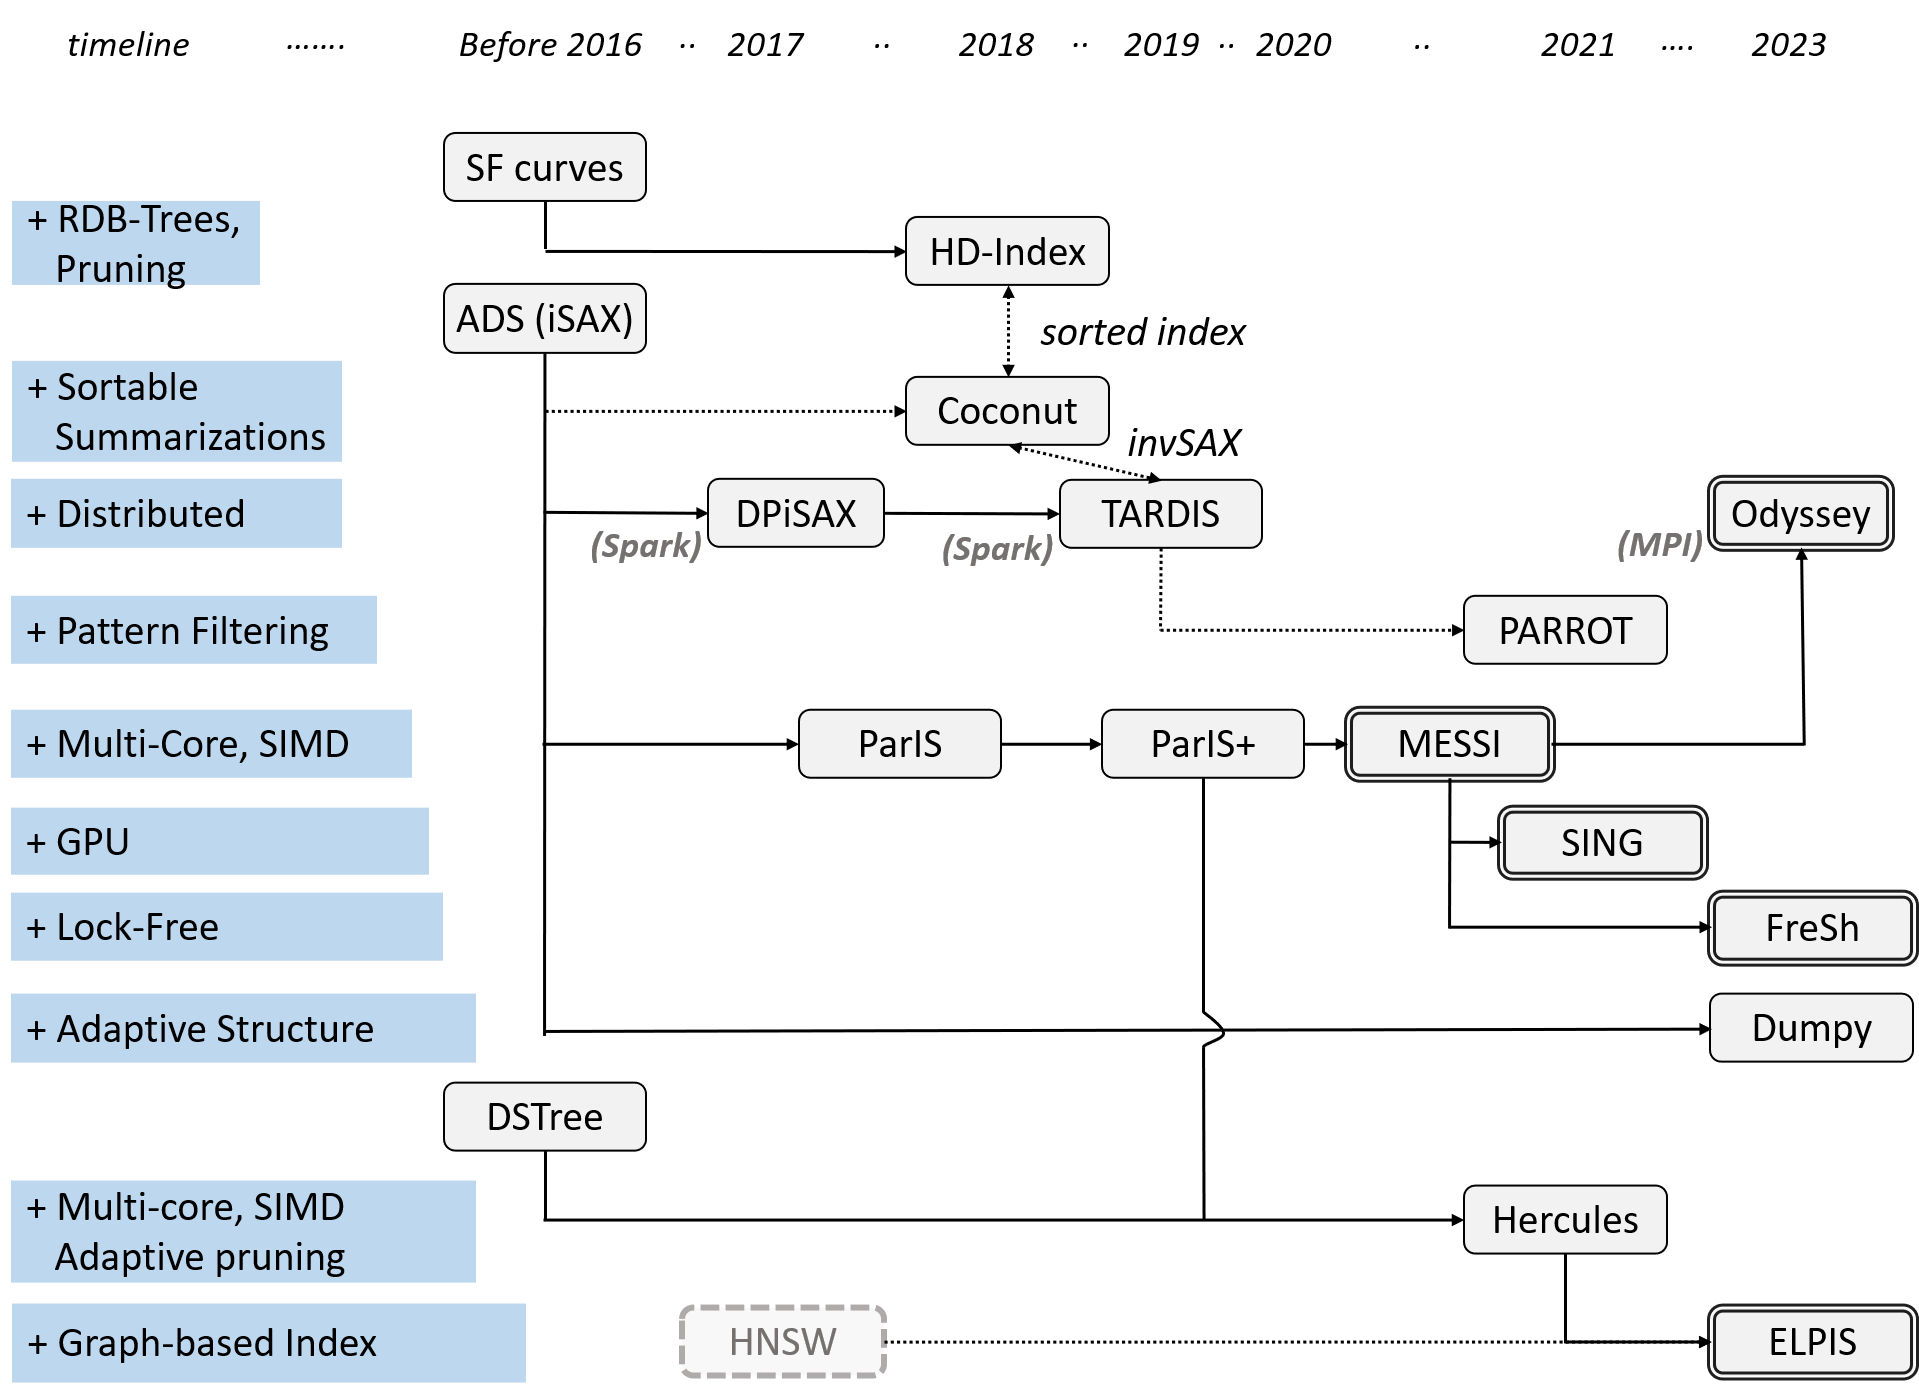
\includegraphics[width=0.8\textwidth]{submissions/Zeyu2023/figs/tree-evo.png}
    \caption{
    %zeyu: add Elpis
    The evolution of tree-based index in the past 6 years, as an extended figure of~\cite{evolution}. The solid arrows denote the inheritance of the index design; the dashed arrows denote the correlation of the design features; indexes in double-lined boxes are in-memory solutions, while the rest are on-disk solutions. Note that HNSW is not a tree-based index; it is included, because ELPIS (discussed in Section~\ref{zeyu_sec:combination}) inherits some of its features.}
    \label{zeyu_fig:evo-tree}
\end{figure}

\subsection{Optimized Disk Index Structure}
Managing large-scale high-dimensional vectors on disk is challenging since the data locality (i.e., similar vectors should be placed together such that they can be fetched by one I/O) and the index quality (i.e., nearest neighbors should be quickly located by the index) should be considered at the same time.
% Most advanced works before the following recent progress, like iSAX2+~\cite{isax2+} need days to index billion-level data and minutes to execute a query.
Recent progress has remarkably advanced the state-of-the-art to hour-level indexing time and ms-level query time on billion-sized datasets.

% zeyu: shortened
\paragraph{HD-Index~\cite{hd-index}.}
HD-Index, as an ordered index, builds multiple B+ trees each of which stores the Hilbert keys of a segment of dimensions.
In this way, HD-Index mitigates the loss of accuracy due to the dimensionality reduction.
To facilitate the refinement, HD-Index randomly places pivots and stores in the index the distance between an entry and the nearest reference point, which provides the ability to prune when querying.
However, the search cost of HD-Index increases linearly with dimensionality, leading to an inefficient solution for very high-dimensional vectors.

% zeyu: I'd like to discuss Coconut again for its prominent merits and defects.
\paragraph{Coconut~\cite{coconut}.}
In contrast to HD-Index which sorts raw (sub)-vectors, Coconut first reduces dimensionality using SAX, and then sorts SAX words by the z-order curve.
In this way, the most significant dimensions (i.e., bits) of the SAX words are considered first.
This process matches exactly the principle of SAX summarization, i.e., coarse-grained partitioning is encoded in the most significant bits, while fine-grained partitioning in the least significant bits. 
Using only one B-tree to index the keys, Coconut has a very fast query time, and the highly packed leaves also lead to a small improvement in the results of approximate search.
%However, as Coconut does not implement any special approximate search algorithm, it is hard to achieve a high recall with a limited number of candidates.

\paragraph{Dumpy~\cite{dumpy}.}
Dumpy is an iSAX-based index designed for high-precision approximate search and fast index-building for large datasets.
Dumpy leverages the trade-off between the proximity inside the leaf node and the compactness (i.e., the fill factor) of these nodes by dynamically selecting the number of segments and which segments to split along according to the data distribution.
It also proposes a leaf node packing algorithm and a vector duplication mechanism that further optimizes the data layout on the index.
As a result, Dumpy can provide high-recall answers with much fewer random I/Os. % with the preserved pruning ability of iSAX.


\subsection{Parallel Processing}
Parallel indexing and querying on the tree-based index is not trivial for dynamic structure and pruning-based query~\cite{paris,messi}.
The difficulties include the reduction of race conditions and load balancing among threads.
The ParIS+ index~\cite{paris}, parallelizes the building and querying algorithms of ADS+~\cite{ads}, an adaptive variant of the iSAX index.
MESSI~\cite{messi} further optimizes the race conditions for in-memory datasets, while SING~\cite{sing} extends the query answering algorithm to make use of GPUs.
In recent years, the research boundary has been pushed by a parallel and fully-materialized disk index, and a novel lock-free parallelism mechanism.


\paragraph{Hercules~\cite{hercules}.}
Hercules is an EAPCA-based parallel disk-based index.
Designed for large-scale datasets, Hercules optimizes memory management with a two-level buffer model to reduce the time cost of memory management.
Besides that, Hercules delicately schedules different tasks with a given number of threads, resulting in (1) CPU-intensive tasks being executed in parallel to I/O-intensive tasks, (2) the number of I/Os being significantly reduced, and (3) avoiding race conditions.
Moreover, Hercules proposes a composite query algorithm with hierarchical pruning by different distance approximations.
Being the first parallel dynamic (EAPCA-based) tree index, Hercules shows robust and remarkable index-building and query answering performance improvements. % beyond sequential index building and querying algorithms.
(Hercules also inherits properties to ELPIS~\cite{elpis}, a parallel in-memory index for approximate search, which we discuss in Section~\ref{zeyu_sec:combination}.)

\paragraph{FreSh~\cite{fresh}.}
FreSh is an iSAX-based parallel in-memory index, proposing a novel lock-free approach for building and querying the index.
FreSh modularizes iSAX-based indexes, and parallelizes the tasks of these modules under Refresh, a generic framework that can be applied on top of any locality-aware data series algorithm to ensure lock-freedom.
FreSh also designs a helping mechanism with a small synchronization cost for load balancing among threads.
The combination of the tree-based index and lock-free mechanism opens more directions for improving the parallelism of tree-based indexes.

\subsection{Distributed Processing}
The core challenges of distributed indexes are how to place the dataset into different machines, how to achieve load balancing among these machines, and how to coordinate these machines to serve queries. 
The previous study in this area, i.e., DPiSAX~\cite{dpisax}, partitions data by the distribution on the SAX space of the sampling data and dispatches queries to corresponding partitions.
Recent studies have advanced it from the aspects of partition quality, load balance, and scalability of indexing and querying, by introducing and designing novel techniques for distributed systems.

\paragraph{TARDIS~\cite{tardis}.}
As an iSAX-based index, the rationale of TARDIS is to cluster similar nodes into the same pack.
The pack is organized as middle-sized and the placement of these packs depends on the downstream distributed file systems (e.g., HDFS).
The clustering is based on a variant of iSAX, invSAX, which places the prior bits into the first positions and then the later bits.
TARDIS prominently advances DPiSAX~\cite{dpisax} by load balancing and cooperative querying.
However, it loses the ability to prune and suffers from the low proximity of data inside a pack, limiting the practicability and the improvement.

\paragraph{PARROT~\cite{parrot}.}
PARROT is built as a secondary index for a partitioned data warehouse.
PARROT identifies patterns by clustering on dimension-reduced SAX space, and stores the distribution of patterns in a global index with exception points.
However, PARROT relies on the existence of a strong correlation pattern between the partition key and the vector inside.
Otherwise, the vectors of the same pattern will distribute sparsely across the data warehouse and querying will deteriorate to a linear scan.

\paragraph{Odyssey~\cite{odyssey}.}
Odyssey is a scalable framework for distributed in-memory data series similarity search in clusters with multi-core servers, thus, exploiting parallelization both inside and across system nodes.
Odyssey follows the classical design principle of horizontal splitting and vertical duplication in distributed systems.
Unlike TARDIS, Odyssey tries to achieve load balancing through carefully partitioning the data across machines (by storing similar series to different machines), assigning queries to machines using a clever scheduling algorithm (by estimating the execution time of each query), and employing more resources for hard queries (by using a light-weight work-stealing technique).
Odyssey also duplicates the data splits across several machines, which enables further parallelization in query answering, as well as load-balancing (through work-stealing).
%Moreover, Odyssey introduces a work-stealing mechanism that helps load balancing among the threads that own the same data splits.
As a result, Odyssey achieves nearly linear scalability on an increasing number of machines, or queries.

\subsection{Discussion}
\label{zeyu_sec:discuss}
From the summarization and analyses above, we can observe that tree-based indexes are developed toward practical, large-scale, parallel, and distributed scenarios.
These extensions fully leverage the data locality and high efficiency of tree-based indexes.
On the other hand, an inherent drawback of the tree-based indexes is that it is hard to overcome the curse of dimensionality.
The similarity between the points in a partition of a tree index is decided by a hyperplane in high dimensions, which usually needs to balance separability and the proximity of the data.
As the height of a tree is limited (which influences the search performance), only limited dimensions and features are considered to form the hyperplane.
Therefore, it is not easy to quickly locate all the nearest neighbors in a tree index.

\section{Comparative Study and Open Directions}
\label{zeyu_sec:compare}
\subsection{Comparison Between Graph- and Tree-based Indexes}
\begin{table}[t]
\centering
\footnotesize
\caption{A comparative study of graph- and tree-based indexes.}
\label{zeyu_tab:compare}
\begin{tabular}{cccc}\toprule
                                  \multicolumn{2}{c}{Comparison Items}                          & Graph            & Tree               \\ \midrule
\multirow{3}{*}[-1.5mm]{Basic Properties} & Rationale               & Navigability     & Space-partitioning \\\cmidrule{2-4}
                                  & Data locality           & $\times$         & $\checkmark$       \\\cmidrule{2-4}
                                  & Dimension reduction     & $\times$         & $\checkmark$       \\\midrule
\multirow{6}{*}[-8mm]{Query Answering} &
  Search pattern &
  Best-first-search &
  Prioritized tree traversal \\\cmidrule{2-4}
                                  & Two-stage search        & $\checkmark$     & $\checkmark$       \\\cmidrule{2-4}
                                  & Navigating stage        & Fast & Fast               \\\cmidrule{2-4}
                                  & Recall stage            & Fast             & Slow               \\\cmidrule{2-4}
                                  & Progressive search   &  $\checkmark$ & $\checkmark$ \\\cmidrule{2-4}
 &
  \begin{tabular}[c]{@{}c@{}}Pruning/ $\epsilon$-accuracy\\ guarantee\end{tabular} &
  $\times$ &
  $\checkmark$ \\\cmidrule{2-4}
 &
  \begin{tabular}[c]{@{}c@{}}Early termination of\\ distance calculation\end{tabular} &
  $\checkmark$ &
  $\checkmark$ \\\midrule
\multirow{2}{*}[-1mm]{Parallelism}      & Index construction      & $\checkmark$     & $\checkmark$       \\\cmidrule{2-4}
                                  & Intra-query parallelism & $\checkmark$     & $\checkmark$       \\\midrule
\multirow{2}{*}[-1mm]{\begin{tabular}[c]{@{}c@{}}Distributed\\ indexing\end{tabular}} &
  Load balance &
  $\times$ &
  $\checkmark$ \\\cmidrule{2-4}
                                  & Query collaboration     & $\times$         & $\checkmark$      \\ \bottomrule
\end{tabular}
\end{table}

As shown in Table~\ref{zeyu_tab:compare}, we compare graph- and tree-based indexes along four dimensions, namely, basic properties, query answering, parallelism, and distributed indexing.

\paragraph{Basic properties.}
The motivations of these two kinds of indexes are different.
Graph-based indexes are motivated by the navigability of a small-world graph model whereas tree-based indexes organize data according to the proximity of neighboring vectors.
Therefore, tree-based indexes group similar vectors together and own data locality while graph-based indexes are not aware of the data locality explicitly.
Since graph-based indexes only use the absolute distance between points for indexing, the dimensions of the vectors are usually ignored and hence no dimension reduction techniques are used, despite that the dimensions of space are impacting the quality of indexes implicitly.
On the contrary, tree-based indexes need to explicitly split the partitions and a high dimensionality will severely impact the quality of splits.
Thus, dimensionality reduction has become the rule of thumb for tree-based indexes.

%\paragraph{Scalability and index update.}
Tree-based indexes can usually be deployed either on disk or in memory, and enjoy cache acceleration by virtue of the data locality.
However, it is hard for graph-based indexes to leverage data locality as they are secondary indexes (i.e., the data is not stored inside the index).
% However, when placing graph-based indexes on disk, the query performance will deteriorate due to frequent random accesses, which significantly limits the scalability of graph-based indexes.
Moreover, inserting a vector into a graph-based index usually means a change in the topology of the graph.
This indicates that ingestion throughput is limited, especially when the graph is large.
Some promising studies propose efficient on-disk solutions~\cite{diskann,spann,grip} and effective update strategies~\cite{freshdiskann} to address these problems, which nevertheless, remain interesting research directions for graph-based indexes.

\paragraph{Query answering.}
As for querying, graph-based indexes follow a best-first-search pattern on the graph, while tree-based indexes find the closest partitions to the query vector by prioritized tree traversal.
Nevertheless, both these two algorithms are reminiscent of two-stage searching~\cite{osdi} (i.e., navigating and recall stages).
For both algorithms, the navigating stage can be very fast while in the recall stage, graph-based indexes are far more efficient than the tree-based ones.
This is because the $k$NN of the candidates are directly linked in the graph index.
On the other hand, the tree-based index provides a bound for the query vector and a group of database vectors, allowing multi-level pruning with no false negatives, which can also be used to build mechanisms that provide (deterministic or probabilistic) guarantees for the approximate search answers~\cite{hydra2,pros}.
On the contrary, graph-based indexes cannot safely prune any of the visited points. 
As a common point, when pruning fails, both graph- and tree-based indexes can early stop the exact distance calculations between the query and the candidate answers (i.e., without having to process all the dimensions)~\cite{adsampling,kdd11}.
Note that while graph-based indexes can only support ANNS (with no quality guarantees), the tree-based indexes discussed in this paper support all flavors of similarity search, ranging from ANNS without and with (probabilistic and deterministic) quality guarantees to exact similarity search. 

%\paragraph{Progressive search.}
Another direction that has been studied in the context of both graph- and tree-based indexes is progressive search~\cite{pros,panene,early-termination,leqat}.
In the recall stage, ANNS tries to answer two questions:
(i) Is the current Best-So-Far (BSF) answer the exact $k$NN?
(ii) If not, when will the exact $k$NN occur?
Note that the answers to these questions are not known during query answering. 
However, estimations of the answers to these questions can benefit the query algorithms.
First, if the answer to the first question is positive, the query algorithm can terminate immediately.
As demonstrated in an earlier study~\cite{pros}, the time needed for ANNS to determine the answer to the first question after having already found the exact $k$NN, corresponds to the vast majority of the total query answering time.
Therefore, an agile termination can significantly accelerate high-precision search.
Recently, ProS~\cite{pros} proposed the use of simple machine learning models to provide various probabilistic quality guarantees (such as, on the current result being the exact $k$NN, the distance of the current answer being less than $\epsilon$ from the exact $k$NN distance, and others) for intermediate (i.e., progressive) results during the query answering process.
Moreover, by answering the second question, we can dynamically schedule the computing resources by controlling the search parameters, such as $ef$, and the number of leaves to visit for a precision target.
To achieve this, for tree-based indexes, ProS uses quantile regression that estimates the $1-\phi$ quantile of the time needed to find the exact answer with the BSF answers.
For graph-based indexes, a recent study~\cite{early-termination} enriches the features by (a) the query itself, (b) the progress made from the start point to the current point, and (c) the ratio of existing features.
With these features, it trains Gradient Boosting Decision Trees for regression.


\paragraph{Parallelism.}
Both kinds of indexes have been extended to support parallelization.
For index construction, tree-based indexes have evolved to the solutions described above, and such parallelism for graph-based indexes is also natural.
For intra-query parallelism, these two kinds of index families also propose corresponding extensions, like Hercules~\cite{hercules}, MESSI~\cite{messi}, SING~\cite{sing}, FreSh~\cite{fresh} and ELPIS~\cite{elpis} for tree-based indexes, and SONG~\cite{song} and iQAN~\cite{iqan} for graph-based indexes.

\paragraph{Distributed indexing.}
While some studies have focused on distributed solutions for tree-based indexes~\cite{dpisax,tardis,parrot,odyssey}, the direction of distributed graph-based indexes has not been studied in depth. 
Existing solutions~\cite{milvus,nsg} use random data partitioning and independent building of the corresponding parts of the index.
Therefore, the computing power of the machines is not fully leveraged, and there are untapped opportunities for improving scalability~\cite{pyramid,leqat}.







\subsection{Existing Combinations of the Two Kinds of Indexes}
\label{zeyu_sec:combination}

In this subsection, we survey the existing solutions that combine these two kinds of indexes and analyze their common points and design principles.

\paragraph{SPTAG~\cite{sptag} and SPANN~\cite{spann}.}
Similar to HVS and LSH-APG, SPTAG adopts a balanced K-means tree~\cite{bkt} to locate better entry points.
While SPANN as a disk index, partitions data by a balanced K-means tree, and each partition is stored sequentially on disk.
The data partitions are further refined by duplication.
To quickly find the nearest partitions, SPANN builds a SPTAG index in memory for the partition centroids.
% In this way, SPANN uses an in-memory graph-based index to find the nearest clusters and refines the vectors in these clusters.
As a result, it shows remarkable improvement compared with dumping an optimized graph into the disk~\cite{diskann}.


\paragraph{LANNS~\cite{lanns} and ELPIS~\cite{elpis}.}
Another family of solutions constructs a tree index to partition the data, and builds a graph within each partition (leaf node).
LANNS uses a learned hyperplane for splitting and a multi-path search in the tree.
ELPIS~\cite{elpis} leverages Hercules~\cite{hercules} to partition the data.
In contrast to LANNS, ELPIS can prioritize the leaf node according to the lower bound distance to the EAPCA of the query.
In this way, ELPIS provides higher intra-query parallelism, leading to a remarkable improvement in query performance on large-scale datasets.
Since the indexing cost of the tree index is lower than a graph index, ELPIS significantly improves indexing efficiency by 3x-8x, and reduces memory consumption by 40\%.
Interestingly, ELPIS shows the trade-off between query efficiency and accuracy when varying the number of partitions.
That is, more partitions improve search efficiency at the expense of accuracy, but there exists a sweet point that optimizes performance.
% Since the routing cost in the tree index of LANNS and Elpis is more slight than the K-means tree in SPANN, we do not need an extra graph-based index for finding 

\paragraph{Discussion.}
So far we have studied three kinds of combinations of graph- and tree-based indexes, including
(1) using the tree index to obtain better entry points for the graph index (HVS, LSH-APG, and SPTAG);
(2) using the graph index to find the closest leaf nodes in the tree index (SPANN);
(3) using the tree index to partition data and building graph indexes on each leaf node (LANNS and ELPIS).
We can deduce the following key ideas from these combinations. 
(i) The tree index can promote the representation granularity from vector-level to node level, even in sub-tree level, which makes it easy to handle large-scale and disk-resident datasets.
(ii) The cases in large-sized datasets (billion-level) are not the same as middle-sized (million-level), where the pros and cons of different index families should be re-considered carefully. 
(iii) The tree index still suffers from the boundary issue and must be adapted to improve the search accuracy (e.g., duplication). 
(iv) It is yet intractable to build the graph index on the whole dataset, while at the same time, the graph index is irreplaceable for achieving high recall efficiently.
Based on these explorations, in the next section, we will introduce more possible directions where tree-based, as well as other kinds of indexes can assist the graph index to overcome more inherent limitations.


% As we have analyzed and extensively verified, graph-based indexes are irreplaceable for the efficiency in recall stage.
% At the same time, there are many problems when using only the graph-based index such as high construction cost, high memory footprint, no accuracy guarantee for approximate search, weak scalability and etc.

% In addition to use tree-based indexes as an auxiliary data structure to acquire better entry points for graph-based indexes, there exist another two ways to combine these two indexes together as described in this section, i.e., 



\subsection{Open Problems and Promising Future Directions}
In this subsection, we propose four open problems that are crucial for solving ANNS problems in practice and at scale. 
More importantly, combining the techniques from the tree- and graph-based index is a promising way to solve these problems. 

\paragraph{Dimension reduction and pruning.}
The most costly operation for graph-based indexes is the distance calculation, reducing dimensions can provide a linear improvement on query~\cite{adsampling}.
For example, by rotating the vectors in the directions of the principal component vectors, the early termination mechanisms can behave more efficiently as most of the variations are concentrated in the first dimensions.
The results are shown in Figure~\ref{zeyu_fig:pca}, where the query time is reduced to \textbf{50}\% with this simple optimization.
% It demonstrates that vector-level pruning with appropriate dimension reduction still has a large improvement space that is under exploration.
Moreover, representation learning is also a promising way of embedding high-dimensional vectors in a low-dimensional space. % with the loss of reconstruction error.
A lower bound of the distance measure in the embedded space is often designed at the same time, in order to safely perform pruning.
As demonstrated by GRAIL~\cite{grail} and SEAnet~\cite{seanet}, representation learning is more flexible in capturing the ``shape'' of high-dimensional vectors than traditional methods, because it can adapt to the data at hand.
Similar data-adaptive techniques have been studied in the context of quantization~\cite{vaq,lvq}.
Besides that, inspired by the hierarchical structure of tree-based indexes, after dimension reduction (or rotation, projection), it would be helpful if different vectors can be summarized with a common representation and be safely pruned, i.e., through node-level pruning.
\begin{wrapfigure}{r}{0.5\textwidth}
\centering
\includegraphics[width=0.75\linewidth]{submissions/Zeyu2023/figs/ann-bulletin-gist.png}
\caption{Early termination techniques in HNSW on Gist1M. ADS~\cite{adsampling} is the state-of-the-art technique.}
\label{zeyu_fig:pca}
\end{wrapfigure}
% \begin{wrapfigure}{r}{0.65\textwidth}
% \subfloat[Gist1M]{
% \includegraphics[width=0.48\linewidth]{figs/ann-bulletin-gist.png}
% }
% \subfloat[MNIST]{
% \includegraphics[width=0.48\linewidth]{figs/ann-bulletin-mnist.png}
% }
% \caption{Improve HNSW by more efficient early termination of distance calculation. ADSampling (ADS for short) is the state-of-the-art early termination techniques. PCA is to rotate the dataset by PCA first.}
% \label{zeyu_fig:pca}
% \end{wrapfigure}



% In this way, the $\epsilon$ accuracy guarantee would also become possible.

\paragraph{Distributed indexing.}
% Unlike tree-based indexes that are naturally could be split into disjoint parts, the splitting of graph-based indexes severely degrades the overall query performance compared with indexing on a single complete dataset.
% Moreover, there is no load balancing techniques that could balance the jobs among different machines like Odyssey.
% Besides, the duplication of splits and the collaboration scheme of different machines for efficient querying remain technical challenges for graph-based indexes.
Distributed indexing is a must for managing large-scale high-dimensional data in production.
Distributed tree-based indexes, like Odyssey, have been designed for exact $k$NN search; their ANNS performance can be further improved. % whose efficiency is not satisfactory ($<200$ QPS).
On the other hand, partitioning a graph index is inherently difficult since it is not evident how to partition the graph with load-balanced partitions.
% A naive random splitting degrades the overall performance.
As demonstrated in ~\cite{leqat}, combining the results from multiple disjoint graph indexes split at random is sub-optimal for this problem, and other clustering algorithms like k-means, suffer from imbalance problems.
Therefore, designing a load-balance-oriented data partition scheme that minimizes the loss of efficiency will provide substantial improvements to vector database performance~\cite{milvus,adbv,pinecone}.
In this case, a promising direction is to leverage the space-partitioning scheme of tree-based indexes for splitting data, while estimating the load of each split dynamically, in order to provide more opportunities for collaborative (parallel) work during query answering time. 

\paragraph{Reliable ANNS.}
Current ANNS algorithms are not reliable.
In different datasets (similar cardinality and dimensionality), the search performance is significantly different.
For example, to achieve 90\% recall@20 on HNSW, the search cost is 90x larger for Glove dataset than Deep1M dataset.
Such a result is not a special case~\cite{tau,adsampling,promise,note}.
The reason is closely related to our analyses in Section~\ref{zeyu_sec:graph}.
Although HNSW removes the hubs and mitigates the skewness, the effect of these techniques actually depends on the distribution of the original dataset.
If the distribution of the original dataset is very skewed, the phenomenon that hubs are clustered to trap the search route occurs again in HNSW.
It means that the high efficiency for navigation, and the high local proximity for recalling no longer exist in graph-based indexes.
To further mitigate the skewness, it will be helpful to use (approximate) range search to further filter edges.
It is possible to remove the bias on the nodes with high $k$-occurrence and provide a robust performance over datasets of any distribution.
% This becomes the root cause of the loss of the robustness.
% todo: connectivity of GT in k-Graph

\paragraph{Reliable benchmarks.}
With the rapid growth of the ANNS area, the development of appropriate benchmarks is urgently required, in order to evaluate the solutions based on the different index families we outlined earlier, as well as new solutions that combine and extend the ideas of existing techniques.
Some works in the literature~\cite{hydra1,hydra2,tkde-survey} have been pioneering in this respect, but the latest techniques are not included in them.
Other benchmarks such as~\cite{competition} and~\cite{ann-benchmark,lid} provide an open framework to evaluate the performance of different ANNS algorithms.
However, many engineering tricks can be added to improve the literal performance which on the other hand, might confuse readers without detailed ablation studies.
Moreover, common public datasets such as Sift~\cite{sift}, Gist~\cite{sift}, Deep~\cite{deep}, were produced over a decade ago representing the application of ANNS in the machine learning era.
As the model architecture has evolved significantly in the past decade, it would be beneficial to produce and use newer datasets that correspond to modern applications (e.g., Transformer-based models).

Furthermore, it would be interesting to assess the difficulty of similarity search queries: the different difficulty levels represented by various datasets, as well as various queries on the same dataset, have been observed in the literature~\cite{hardness,lid}. 
However, we still lack a comprehensive analysis and theoretical characterization of the difficulty level of datasets and queries alike, which directly affect the performance of the various indexing approaches, and may also lead to biased evaluation results.
Previous work has studied local intrinsic dimensionality~\cite{lid}, as well as measures related to the tightness of lower bound and data distribution~\cite{hardness}, in order to evaluate the difficulty of a query and a dataset, or more precisely, of a query with respect to a given dataset.
These approaches study the difficulty of pruning candidate points in the dataset, in response to a given $k$NN query. 
% LID and similar pruning-based measures are effective to indicate the difficulty of a query on space-partitioning-based indexes~\cite{hardness}, but not on graph-based indexes~\cite{lid}.
% The reason is two-fold: 
% (1) The rationale of the graph-based index is connectivity instead of distance-based clustering, and thus the distance-based pruning cannot capture the difficulty of connecting the graph
% % (1) Graph-based indexes do not cluster data, or prune irrelevant data based on distance. 
% (2) Due to the randomness of graph-based indexes, the same query will have different difficulties when building the index with different order to insert~\cite{hnsw,shuffle} or refine~\cite{nsg} the vectors in the dataset.
Nevertheless, more extensive and comprehensible studies and benchmarks are needed to more accurately and fairly characterize and evaluate the performance of different ANNS indexes. 
% Previous work~\cite{hardness,lid} describes it by the difficulty of pruning other points from $k$NN, which might be ineffective for graph-based indexes. 

\section{Conclusions}
\label{zeyu_sec:conclude}
In this paper, we study the evolution of the graph-based index family with ablation studies and observe that the keys to its success lie in the randomization and the RNG-based pruning rule.
These techniques preserve the local proximity with fewer edges while building effective long-range connections to enhance navigability. 
We also survey the recent progress of the tree-based index family and discuss their relationships.
Moreover, we conduct a comparative study over these two index families and observe that several of these techniques can complement each other in solving practical problems in ANNS. 
Finally, we point to some interesting research directions in the context of ANNS.

% less than two pages
\begin{thebibliography}{10}
\itemsep=1pt
\begin{footnotesize}
\bibitem{openai} OpenAI. \newblock  Chatgpt-retrieval-plugin. \newblock  {\em \url{https://github.com/openai/chatgpt-retrieval-plugin}}, Accessed Sep. 3, 2023.
\bibitem{postgres}Pgvector. \newblock  \url{https://github.com/pgvector/pgvector/} \newblock  Accessed Sep. 4, 2023.
\bibitem{pinecone}Pinecone. \newblock  \url{https://www.pinecone.io/} \newblock  Accessed Sep. 4, 2023.
\bibitem{scikit-leran}Scikit-learn: Machine Learning in Python. \newblock \url{https://scikit-learn.org/} \newblock  Accessed Sep. 4, 2023.
\bibitem{deep}Skoltech Computer Vision. \newblock  Deep Billion-Scale Indexing. \newblock  {\em \url{http://sites.skoltech.ru/compvision/noimi}}, 2018.  
\bibitem{sift}TEXMEX Research Team. \newblock  Datasets for Approximate Nearest Neighbor Search. \newblock  {\em \url{http://corpus-texmex.irisa.fr/}}, 2018.  
\bibitem{lvq}C.~Aguerrebere, I.~Bhati, M.~Hildebrand, M.~Tepper and T.~Willke. \newblock  Similarity Search In The Blink Of An Eye With Compressed Indices. \newblock  {\em PVLDB}, 2023.
\bibitem{focslsh}A.~Andoni and P.~Indyk. \newblock  Near-optimal Hashing Algorithms for Approximate Nearest Neighbor in High Dimensions. \newblock  {\em FOCS}, 2006.
\bibitem{hd-index}A.~Arora, S.~Sinha, P.~Kumar, and A.~Bhattacharya. \newblock  Hd-index: Pushing The Scalability-accuracy Boundary For Approximate KNN Search In High-dimensional Spaces. \newblock  {\em PVLDB}, 2018.
\bibitem{lid}M.~Aumüller and M.~Ceccarello. \newblock  The Role of Local Dimensionality Measures in Benchmarking Nearest Neighbor Search. \newblock  {\em Inform. Syst.}, 2021.
\bibitem{ann-benchmark}M.~Aumüller, E.~Bernhardsson and A.~Faithfull. \newblock  ANN-Benchmarks: A Benchmarking Tool For Approximate Nearest Neighbor Algorithms. \newblock  {\em Inform. Syst.}, 2020.
\bibitem{ball-tree}L.~Cayton. \newblock   Fast Nearest Neighbor Retrieval for Bregman Divergences. \newblock  {\em ICML}, 2008.  
\bibitem{odyssey}M.~Chatzakis, P.~Fatourou, E.~Kosmas, T.~Palpanas, and B.~Peng. \newblock  Odyssey: A Journey In The Land of Distributed Data Series Similarity Search. \newblock  {\em PVLDB}, 2023.
\bibitem{openqa} D.~Chen, A.~Fisch, J.~Weston, and A.~Bordes. \newblock  Reading Wikipedia to Answer Open-domain Questions. \newblock  {\em ACL}, 2017.
\bibitem{spann} Q.~Chen, B.~Zhao, H.~Wang, M.~Li, C.~Liu, Z.~Li, M.~Yang and J.Wang \newblock  SPANN: Highly-efficient Billion-scale Approximate Nearest Neighbor Search. \newblock  {\em NeurIPS}, 2021.
\bibitem{sptag}Q.~Chen, H.~Wang, M.~Li, G.~Ren, S.~Li, J.~Zhu, J.~Li, C.~Liu, L.~Zhang, and J.~Wang. \newblock  SPTAG: A Library for Fast Approximate Nearest Neighbor Search. \newblock  \url{https://github.com/Microsoft/SPTAG}, 2018.
\bibitem{finger}P.~Chen, W.~Chang, J.~Jiang, H.~Yu, I.~Dhillon, and C.~Hsieh \newblock  FINGER: Fast Inference for Graph-based Approximate Nearest Neighbor Search. \newblock  {\em WWW}, 2023.  
\bibitem{10.1145/1242572.1242610} A.~Das, M.~Datar, A.~Garg, and S.~Rajaram. \newblock  Google News Personalization: Scalable Online Collaborative Filtering. \newblock  {\em WWW}, 2007.
\bibitem{nn-descent}W.~Dong, C.~Moses, and K.~Li. \newblock Efficient K-nearest Neighbor Graph Construction for Generic Similarity Measures \newblock  {\em WWW}, 2011.
\bibitem{lanns}I.~Doshi, D.~Das, A.~Bhutani, R.~Kumar, R.~Bhatt, and N.~Balasubramanian. \newblock LANNS: A Web-scale Approximate Nearest Neighbor Lookup System. \newblock  {\em PVLDB}, 2022.
\bibitem{pyramid}S.~Deng, X.~Yan, K.~Kelvin, C.~Jiang, and J.~Cheng. \newblock Pyramid: A General Framework for Distributed Similarity Search on Large-scale Datasets. \newblock  {\em BIGDATA}, 2019.
\bibitem{hercules}K.~Echihabi, P.~Fatourou, K.~Zoumpatianos, T.~Palpanas, and H.~Benbrahim. \newblock Hercules Against Data Series Similarity Search. \newblock  {\em PVLDB}, 2022.
\bibitem{elpis}K.~Echihabi, K.~Zoumpatianos, and T.~Palpanas. \newblock ELPIS: Graph-Based Similarity Search for Scalable Data Science. \newblock  {\em PVLDB}, 2023.  
\bibitem{hydra2}K.~Echihabi, K.~Zoumpatianos, T.~Palpanas, and H.~Benbrahim. \newblock Return of The Lernaean Hydra: Experimental Evaluation of Data Series Approximate Similarity Search. \newblock  {\em PVLDB}, 2019.
\bibitem{hydra1}K.~Echihabi, K.~Zoumpatianos, T.~Palpanas, and H.~Benbrahim. \newblock The Lernaean Hydra of Data Series Similarity Search: An Experimental Evaluation of the State Of The Art. \newblock  {\em PVLDB}, 2018.
\bibitem{fresh}P.~Fatourou, E.~Kosmas, T.~Palpanas and G.~Paterakis. \newblock  FreSh: A Lock-Free Data Series Index. \newblock  {\em SRDS}, 2023.
\bibitem{dist-concentrate}D.~Francois, V.~Wertz, and M.~Verleysen. \newblock The Concentration of Fractional Distances. \newblock  {\em TKDE}, 2007.  
\bibitem{efanna}C.~Fu and D.~Cai. \newblock EFANNA: An Extremely Fast Approximate Nearest Neighbor Search Algorithm Based on kNN Graph. \newblock  {\em arXiv}, 2016.
\bibitem{nsg}C.~Fu, C.~Xiang, C.~Wang, and D.~Cai. \newblock Fast Approximate Nearest Neighbor Search with The Navigating Spreading-out Graph. \newblock  {\em PVLDB}, 2019.
\bibitem{nssg}C.~Fu, C.~Wang, and D.~Cai. \newblock High Dimensional Similarity Search with Satellite System Graph: Efficiency, Scalability, and Unindexed Query Compatibility. \newblock  {\em TPAMI}, 2021.
\bibitem{adsampling}J.~Gao, and C.~Long. \newblock High-dimensional Approximate Nearest Neighbor Search: with Reliable and Efficient Distance Comparison Operations. \newblock  {\em SIGMOD}, 2023.
\bibitem{pros}A.~Gogolou, T.~Tsandilas, K.~Echihabi, A.~Bezerianos, and T.~Palpanas. \newblock  ProS: Data Series Progressive k-NN Similarity Search and Classification with Probabilistic Quality Guarantees. \newblock  {\em VLDBJ}, 2023.
\bibitem{pmlr-v119-guu20a} K.~Guu, K.~Lee, Z.~Tung, P.~Pasupat, and M.~Chang. \newblock Retrieval Augmented Language Model Pre-training. \newblock  {\em PMLR}, 2020.
\bibitem{k-regular}N.~Hezel, K.~Barthel, K.~Schall, and K.~Jung. \newblock Fast Approximate Nearest Neighbor Search with a Dynamic Exploration Graph Using Continuous Refinement. \newblock  {\em arXiv}, 2023.
\bibitem{panene}J.~Jo, J.~Seo, and J.~Fekete. \newblock PANENE: A Progressive Algorithm for Indexing and Querying Approximate K-Nearest Neighbors. \newblock  {\em TVCG}, 2018.  
\bibitem{faiss}J.~Johnson, M.~Douze, and H.~J{\'e}gou. \newblock Billion-scale Similarity Search with GPUs. \newblock  {\em TBD}, 2019.
\bibitem{coconut}H.~Kondylakis, N.~Dayan, K.~Zoumpatianos, and T.~Palpanas. \newblock Coconut: A Scalable Bottom-up Approach for Building Data Series Indexes. \newblock  {\em PVLDB}, 2018.
\bibitem{learnedanns}M.~Li, Y.~Zhang, Y.~Sun, W.~Wang, I.~W.~Tsang and X.~Lin. \newblock {I/O} Efficient Approximate Nearest Neighbour Search Based on Learned Functions. \newblock  {\em ICDE}, 2020.
\bibitem{pdci}K.~Li and J.~Malik. \newblock  Fast k-nearest Neighbour Search via Prioritized {DCI}. \newblock  {\em ICML}, 2017.
\bibitem{li2022survey} H.~Li, Y.~Su, D.~Cai, Y.~Wang, and L.~Liu. \newblock A Survey on Retrieval-Augmented Text Generation. \newblock  {\em arXiv}, 2022.
\bibitem{tkde-survey}W.~Li, Y.~Zhang, Y.~Sun, W.~Wang, M.~Li, W.~Zhang, and X.~Lin. \newblock Approximate Nearest Neighbor Search on High Dimensional Data — Experiments, Analyses, And Improvement. \newblock  {\em TKDE}, 2019.
\bibitem{early-termination}C.~Li, M.~Zhang, D.~Andersen, and Y.~He. \newblock Improving Approximate Nearest Neighbor Search Through Learned Adaptive Early Termination. \newblock  {\em SIGMOD}, 2020.
\bibitem{promise}P.~Lin and W.~Zhao. \newblock  Graph-based Nearest Neighbor Search: Promises and Failures. \newblock  {\em arXiv}, 2019.
\bibitem{sax}J.~Lin and E.~Keogh. \newblock  A Symbolic Representation of Time Series, with Implications for Streaming Algorithms. \newblock  {\em DMKD}, 2003.
\bibitem{bkt}H.~Liu, Z.~Huang, Q.~Chen, M.~Li, Y.~Fu, and L.~Zhang. \newblock Fast Clustering with Flexible Balance Constraints. \newblock  {\em BIGDATA}, 2018.
\bibitem{shuffle}J.~Liu, Z.~Zhu, J.~Hu, H.~Sun, L.~Liu, L.~Liu, G.~Dai, H.~Yang, and Y.~Wang. \newblock Optimizing Graph-based Approximate Nearest Neighbor Search: Stronger and Smarter. \newblock  {\em MDM}, 2022.  
\bibitem{hvs}K.~Lu, M.~Kudo, C.~Xiao, and Y.~Ishikawa. \newblock HVS: Hierarchical Graph Structure Based on Voronoi Diagrams for Solving Approximate Nearest Neighbor Search. \newblock  {\em PVLDB}, 2022.
\bibitem{hnsw} Y.~Malkov and D.~Yashunin. \newblock  Efficient and Robust Approximate Nearest Neighbor Search Using Hierarchical Navigable Small World Graphs. \newblock  {\em TPAMI}, 2018.
\bibitem{nsw}Y.~Malkov, A.~Ponomarenko, A.~Logvinov, and V.~Krylov. \newblock Approximate Nearest Neighbor Algorithm Based on Navigable Small World Graphs \newblock  {\em Inform Syst}, 2014.
\bibitem{pq} Y.~Matsui, Y.~Uchida, H.~j{\'e}gou, and S.~Satoh. \newblock A Survey of Product Quantization. \newblock  {\em ITE Transactions on Media Technology and Applications}, 2018.
\bibitem{evolution}T.~Palpanas. \newblock  Evolution of A Data Series Index: the iSAX Family of Data Series Indexes. \newblock  {\em CCIS}, 2020.
\bibitem{vaq}J.~Paparrizos, I.~Edian, C.~Liu, A.~J. Elmore and M.~Franklin. \newblock Fast Adaptive Similarity Search Through Variance-Aware Quantization. \newblock  {\em ICDE}, 2022.
\bibitem{grail}J.~Paparrizos and M.~Franklin. \newblock  GRAIL: Efficient Time-series Representation Learning. \newblock  {\em PVLDB}, 2019.
\bibitem{messi}B.~Peng, P.~Fatourou, and T.~Palpanas. \newblock MESSI: In-memory Data Series Indexing. \newblock  {\em ICDE}, 2020.
\bibitem{tau}Y.~Peng, B.~Choi, T.~Chan, J.~Yang, and J.~Xu. \newblock Efficient Approximate Nearest Neighbor Search in Multi-dimensional Databases. \newblock  {\em SIGMOD}, 2023.
\bibitem{sing}B.~Peng, P.~Fatourou, and T.~Palpanas. \newblock SING: Sequence Indexing Using GPUs. \newblock  {\em ICDE}, 2021.
\bibitem{paris}B.~Peng, P.~Fatourou, and T.~Palpanas. \newblock  ParIS+: Data Series Indexing on Multi-core Architectures. \newblock  {\em TKDE}, 2020.
\bibitem{iqan}Z.~Peng, M.~Zhang, K.~Li, R.~Jin and B.~Ren \newblock iQAN: Fast and Accurate Vector Search with Efficient Intra-Query Parallelism On Multi-Core Architectures. \newblock  {\em PPoPP}, 2023.  
\bibitem{hub}M.~Radovanovic, A.~Nanopoulos and M.~Ivanovic. \newblock Nearest Neighbors in High-dimensional Data: the Emergence and Influence of Hubs. \newblock  {\em ICML}, 2009.
\bibitem{kdd11}T.~Rakthanmanon, B.~Campana, A.~Mueen, G.~Batista, B.~Westover, Q.~Zhu, J.~Zakaria, and E.~Keogh. \newblock  Searching and Mining Trillions of Time Series Subsequences Under Dynamic Time Warping. \newblock  {\em KDD}, 2012.
\bibitem{kd-tree}C.~Silpa-Anan and R.~Hartley. \newblock   Optimised KD-trees for Fast Image Descriptor Matching. \newblock  {\em CVPR}, 2008.  
\bibitem{competition}H.~Simhadri, G.~Williams, M.~Aumüller, M.~Douze, A.~Babenko, D.~Baranchuk, Q.~Chen, L.~Hosseini, R.~Krishnaswamy, G.~Srinivasa, S.~Subramanya and J.~Wang. \newblock  Results of the NeurIPS'21 Challenge on Billion-scale Approximate Nearest Neighbor Search. \newblock  {\em NeurIPS (Competition and Demos)}, 2021.
\bibitem{freshdiskann}A.~Singh, S.~Subramanya, R.~Krishnaswamy, and H.~Simhadri \newblock FreshDiskANN: A Fast and Accurate Graph-Based ANN Index for Streaming Similarity Search. \newblock  {\em arXiv}, 2021.  
\bibitem{diskann}S.~Subramanya, Devvrit, R.~Kadekodi, R.~Krishaswamy and H.~Simhadri. \newblock DiskANN: Fast Accurate Billion-point Nearest Neighbor Search on A Single Node. \newblock  {\em NeurIPS}, 2021.
\bibitem{rng}G.~Toussaint. \newblock  The Relative Neighbourhood Graph of A Finite Planar Set. \newblock  {\em Pattern recognition}, 1980.  
\bibitem{milvus}J.~Wang, X.~Yi, R.~Guo, H.~Jin, P.~Xu, S.~Li, X.~Wang, X.~Guo, C.~Li, X.~Xu, K.~Yu, Y.~Yuan, Y.~Zou, J.~Long, Y.~Cai, Z.~Li, Z.~Zhang, Y.~Mo, J.~Gu, R.~Jiang, Y.~Wei, C.~Xie. \newblock Milvus: A Purpose-built Vector Data Management System. \newblock  {\em SIGMOD}, 2021.
\bibitem{dumpy}Z.~Wang, Q.~Wang, P.~Wang, T.~Palpanas, and W.~Wang. \newblock Dumpy: A Compact and Adaptive Index for Large Data Series Collections. \newblock  {\em SIGMOD}, 2023.
\bibitem{note}H.~Wang, Z.~Wang, W.~Wang, Y.~Xiao, Z.~Zhao, and K.~Yang. \newblock A Note on Graph-based Nearest Neighbor Search. \newblock  {\em arXiv}, 2020.
\bibitem{wang-survey}M.~Wang, X.~Xu, Q.~Yue, and Y.~Wang. \newblock A Comprehensive Survey and Experimental Comparison of Graph-based Approximate Nearest Neighbor Search. \newblock  {\em PVLDB}, 2021.
\bibitem{seanet}Q.~Wang and T.~Palpanas. \newblock  SEAnet: A Deep Learning Architecture for Data Series Similarity Search. \newblock  {\em TKDE}, 2023.
\bibitem{dstree}Y.~Wang, P.~Wang, J.~Pei, W.~Wang, and S.~Huang. \newblock A Data-adaptive and Dynamic Segmentation Index for Whole Matching on Time Series. \newblock  {\em PVLDB}, 2013.
\bibitem{adbv}C.~Wei, B.~Wu, S.~Wang, R.~Lou, and C.~Zhan. \newblock  AnalyticDB-V: A Hybrid Analytical Engine towards Query Fusion for Structured and Unstructured data. \newblock  {\em PVLDB}, 2020.
\bibitem{kbs}X.~Xu, M.~Wang, Y.~Wang, and D.~Ma. \newblock Two-stage Routing with Optimized Guided Search and Greedy Algorithm on Proximity Graph. \newblock  {\em KBS}, 2021.
\bibitem{dpisax}D.~Yagoubi, R.~Akbarinia, F.~Masseglia, and T.~Palpanas. \newblock Massively Distributed Time Series Indexing and Querying. \newblock  {\em TKDE}, 2018.
\bibitem{ganns}Y.~Yu, D.~Wen, Y.~Zhang, L.~Qin, W.~Zhang, and X.~Lin. \newblock  GPU-accelerated Proximity Graph Approximate Nearest Neighbor Search and Construction. \newblock  {\em ICDE}, 2022.  
\bibitem{parrot}L.~Zhang, N.~Alghamdi, H.~Zhang, M.~Eltabakh, and E.~Rundensteiner. \newblock PARROT: Pattern-based Correlation Exploitation In Big Partitioned Data Series. \newblock  {\em VLDBJ}, 2022.
\bibitem{osdi}Q.~Zhang, S.~Xu, Q.~Chen, G.~Sui, J.~Xie, Z.~Cai, Y.~Chen, Y.~He, Y.~Yang, F.~Yang, M.~Yang, and L.~Zhou. \newblock {VBASE}: Unifying Online Vector Similarity Search and Relational Queries via Relaxed Monotonicity. \newblock  {\em OSDI}, 2023.
\bibitem{leqat}P.~Zhang, B.~Yao, C.~Gao, B.~Wu, X.~He, F.~Li, Y.~Lu, C.~Zhan, and F.~Tang. \newblock Learning-based Query Optimization for Multi-probe Approximate Nearest Neighbor Search. \newblock  {\em VLDBJ}, 2012.
\bibitem{tardis}L.~Zhang, N.~Alghamdi, M.~Eltabakh, and E.~Rundensteiner. \newblock  TARDIS: Distributed Indexing Framework for Big Time Series Data. \newblock  {\em ICDE}, 2019.
\bibitem{grip}M.~Zhang and Y.~He. \newblock  GRIP: Multi-Store Capacity-Optimized High-Performance
Nearest Neighbor Search for Vector Search Engine. \newblock  {\em CIKM}, 2019.
\bibitem{lsh-apg}X.~Zhao, Y.~Tian, K.~Huang, B.~Zheng, and X.~Zhou. \newblock Towards Efficient Index Construction and Approximate Nearest Neighbor Search in High-dimensional Spaces. \newblock  {\em PVLDB}, 2023.
\bibitem{song}W.~Zhao, S.~Tan, and P.~Li. \newblock  SONG: Approximate Nearest Neighbor Search on GPU. \newblock  {\em ICDE}, 2020.
\bibitem{lsh} B.~Zheng, X.~Zhao, L.~Weng, Q.~Nguyen, H.~Liu, and C.~Jensen. \newblock PM-LSH: A Fast and Accurate In-memory Framework for High-dimensional Approximate NN and Closest Pair Search. \newblock  {\em VLDBJ}, 2021.
\bibitem{ads}K.~Zoumpatianos, S.~Idreos, and T.~Palpanas. \newblock ADS: The Adaptive Data Series Index. \newblock  {\em VLDBJ}, 2016.
\bibitem{hardness}K.~Zoumpatianos, Y.~Lou, I.~Ileana, T.~Palpanas, and J.~Gehrke. \newblock Generating Data Series Query Workloads. \newblock  {\em VLDBJ}, 2018.  
  
\end{footnotesize}
\end{thebibliography}

 \end{document}



